\section{\texorpdfstring{Resolución de la ecuación \(f(x)\  = \ x^{4} - {5x}^{2} - 2x + 1\ \) por medio de la Serie de Fourier.}{Resolución de la ecuación f(x)\textbackslash{}  = \textbackslash{} x\^{}\{4\} - \{5x\}\^{}\{2\} - 2x + 1\textbackslash{}  por medio de la Serie de Fourier.}}\label{resoluciuxf3n-de-la-ecuaciuxf3n-fx-x4---5x2---2x-1-por-medio-de-la-serie-de-fourier.}

\subsection{\texorpdfstring{Braulio Gael Porras Zuñiga }{Braulio Gael Porras Zuñiga }}\label{braulio-gael-porras-zuuxf1iga}

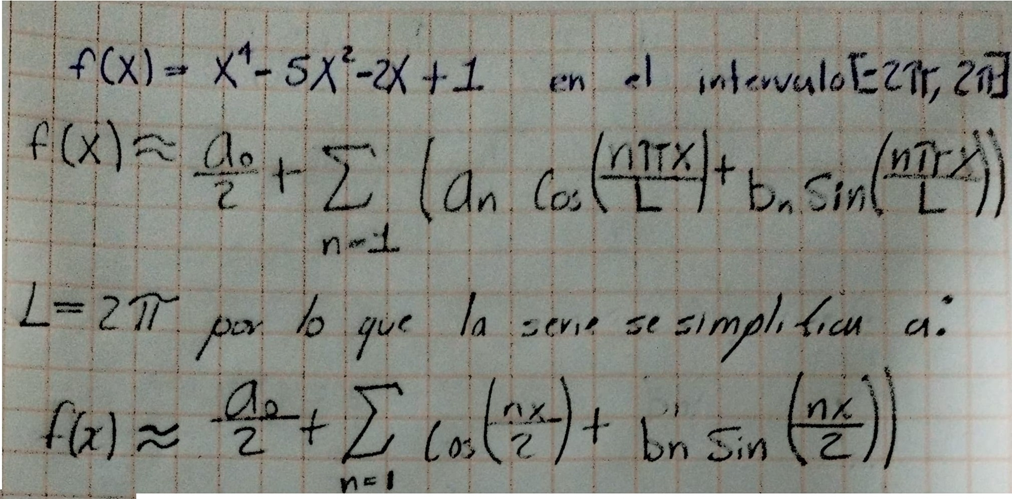
\includegraphics[width=5.15104in,height=2.54129in]{media/image52.png}

Imagen 1A. Procedimiento de Fourier

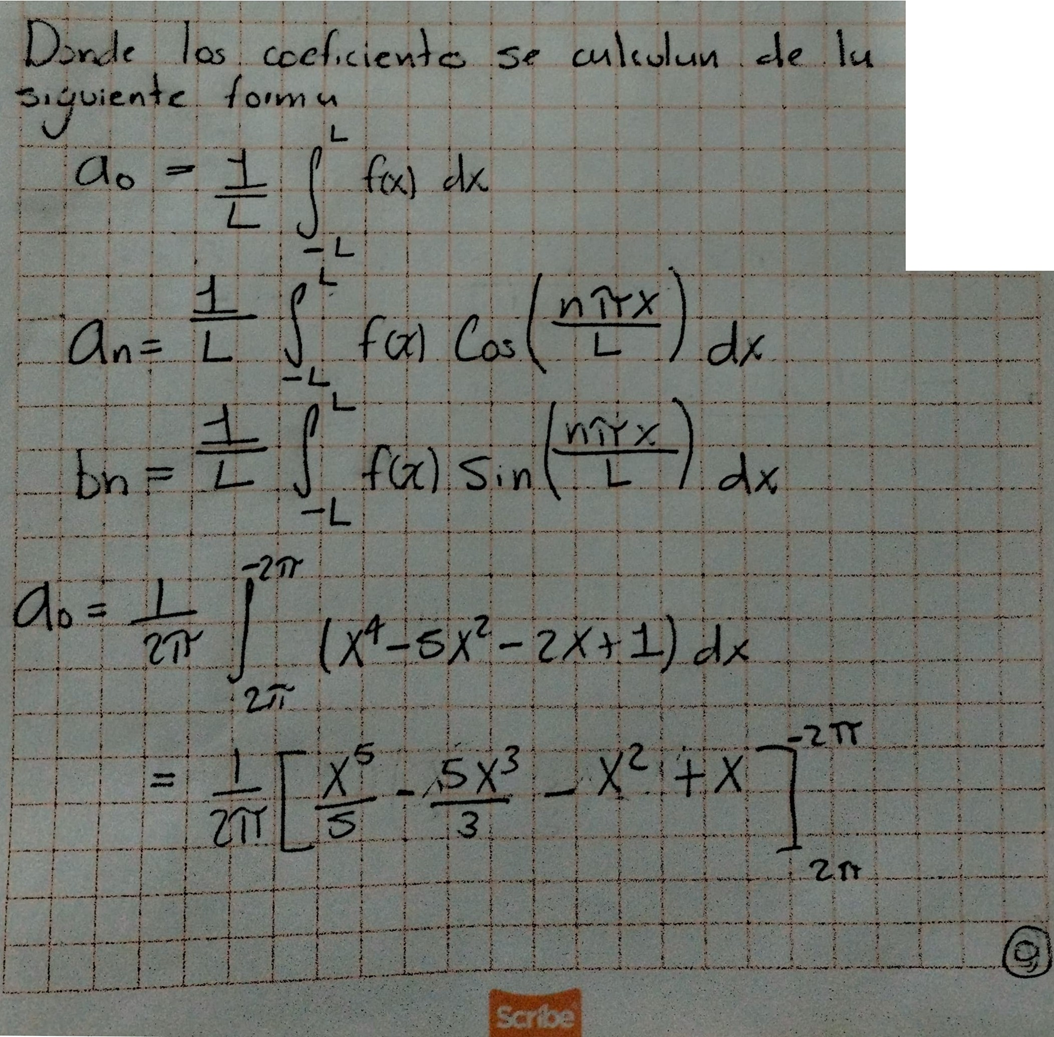
\includegraphics[width=3.66667in,height=3.60643in]{media/image49.png}

Imagen 2A. Procedimiento de Fourier

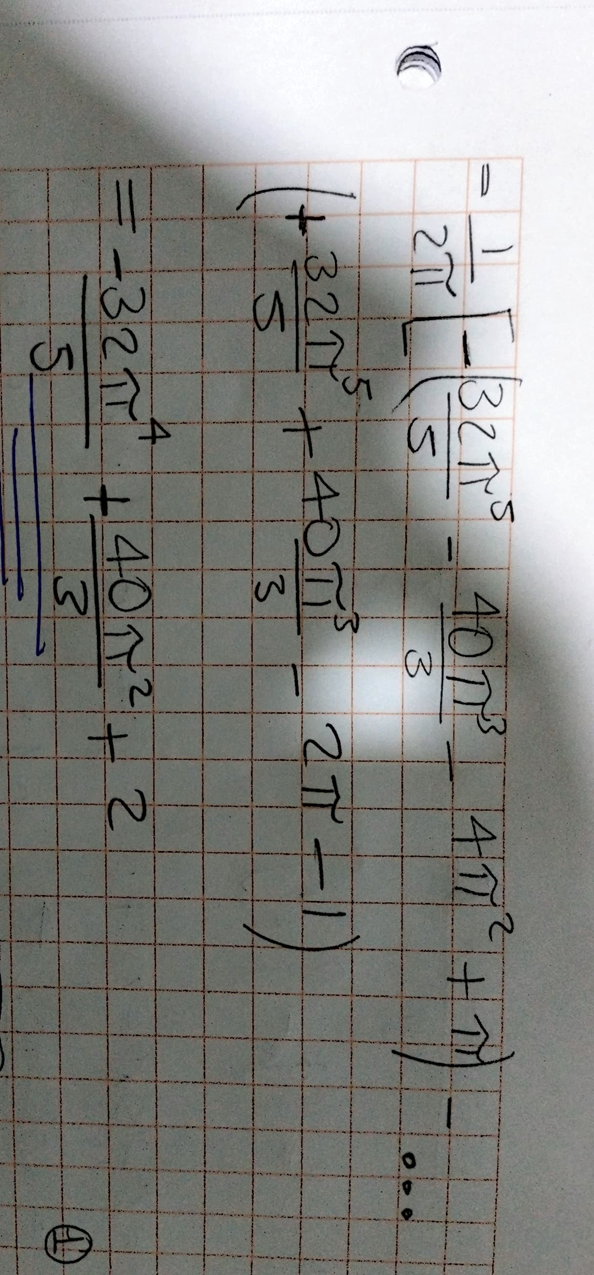
\includegraphics[width=2.34606in,height=5.02604in]{media/image54.png}

Imagen 3A. Procedimiento de Fourier

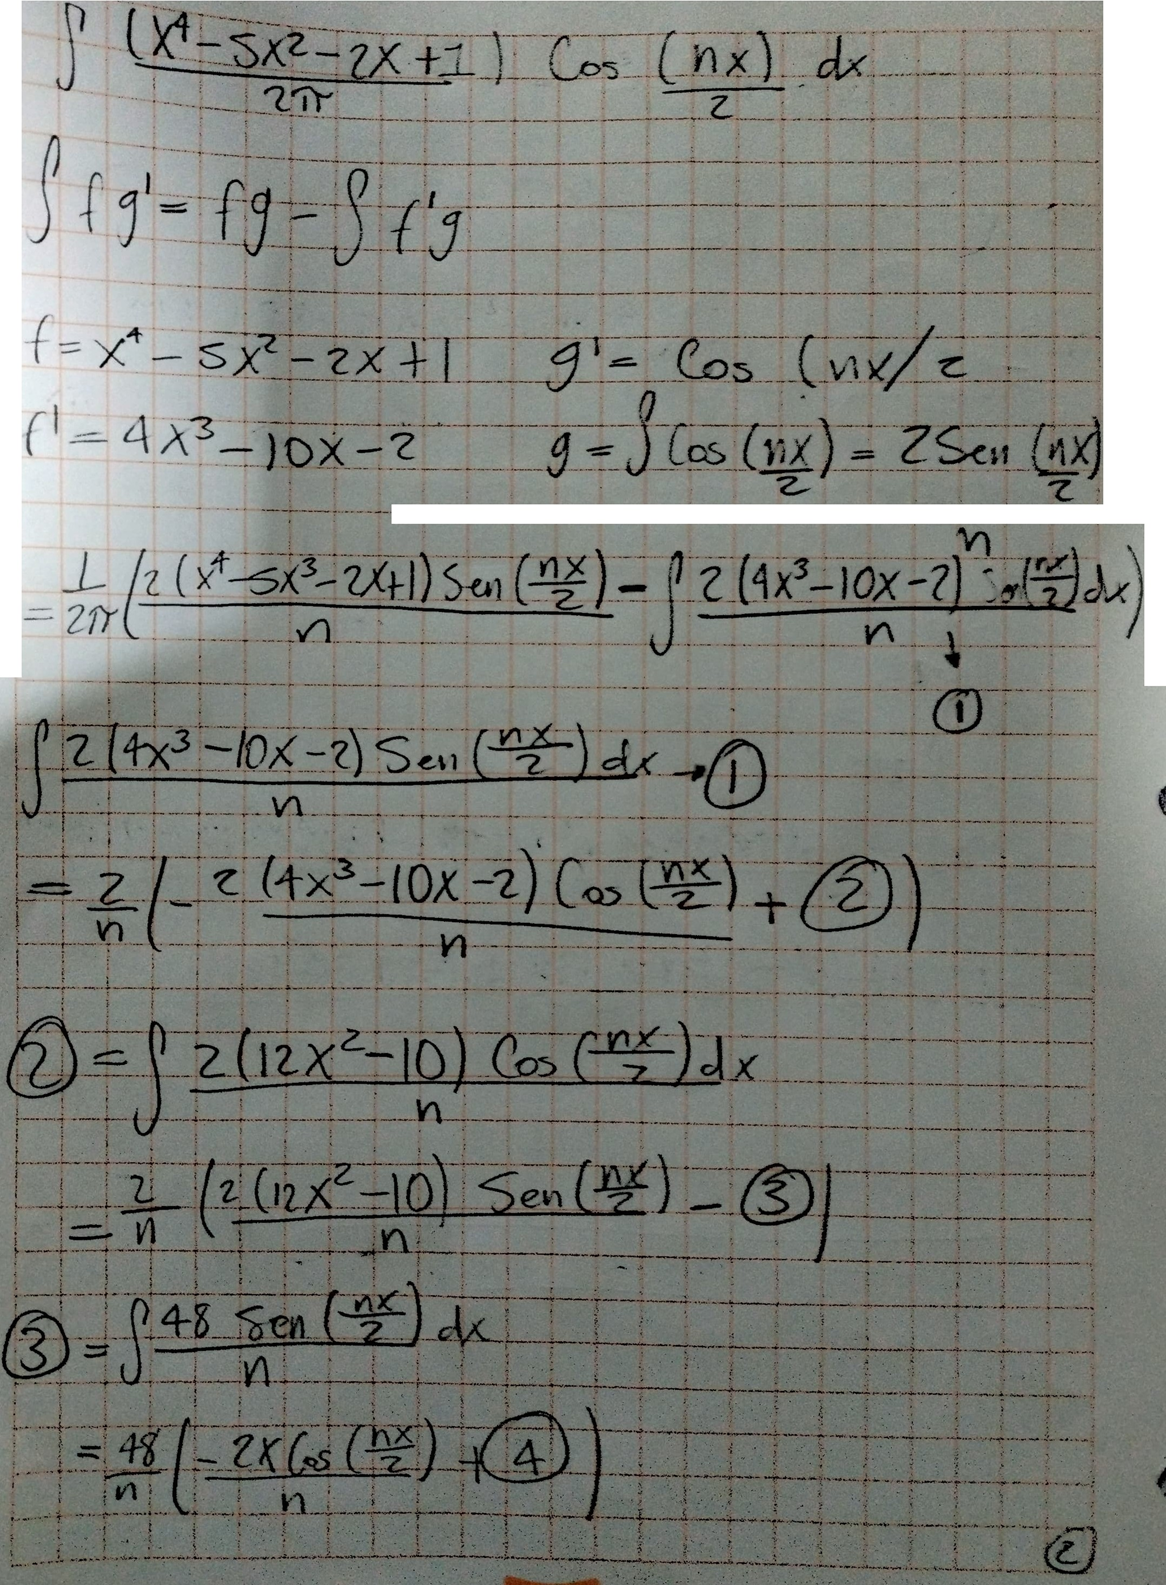
\includegraphics[width=4.84817in,height=6.58854in]{media/image48.png}

Imagen 4A. Procedimiento de Fourier

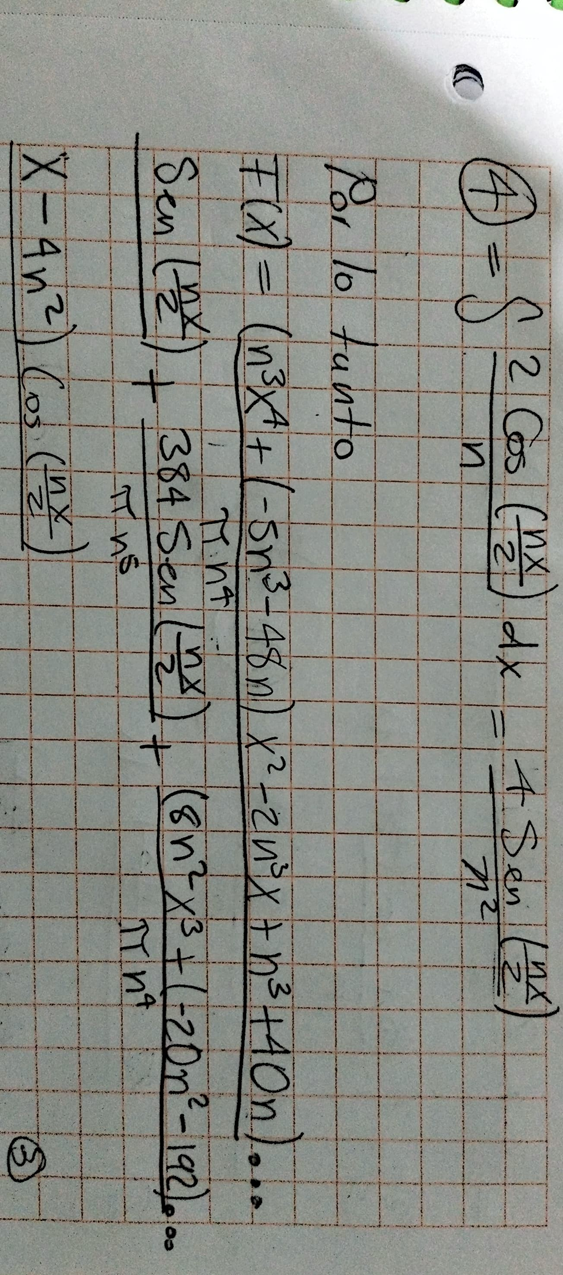
\includegraphics[width=2.15104in,height=4.88023in]{media/image22.png}

Imagen 5A. Procedimiento de Fourier

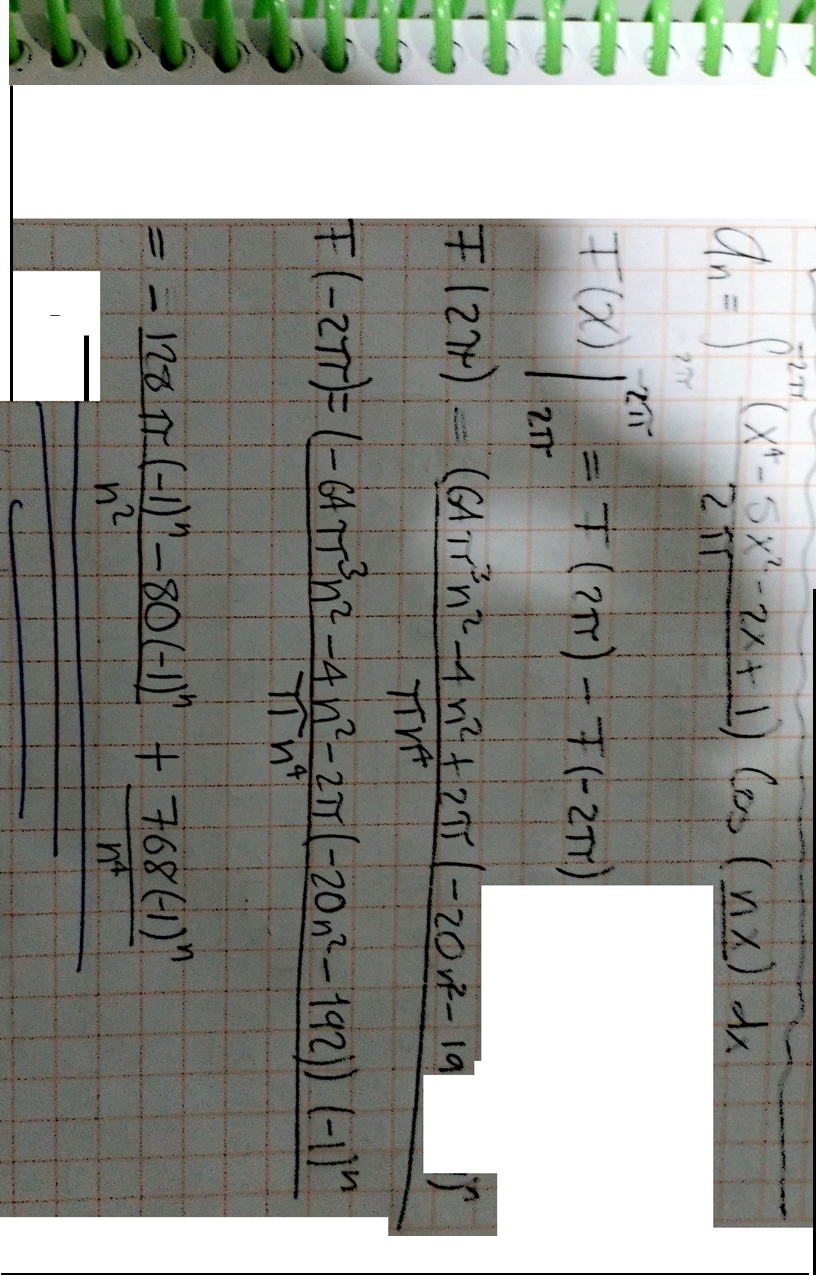
\includegraphics[width=3.07924in,height=4.81771in]{media/image51.png}

Imagen 6A. Procedimiento de Fourier

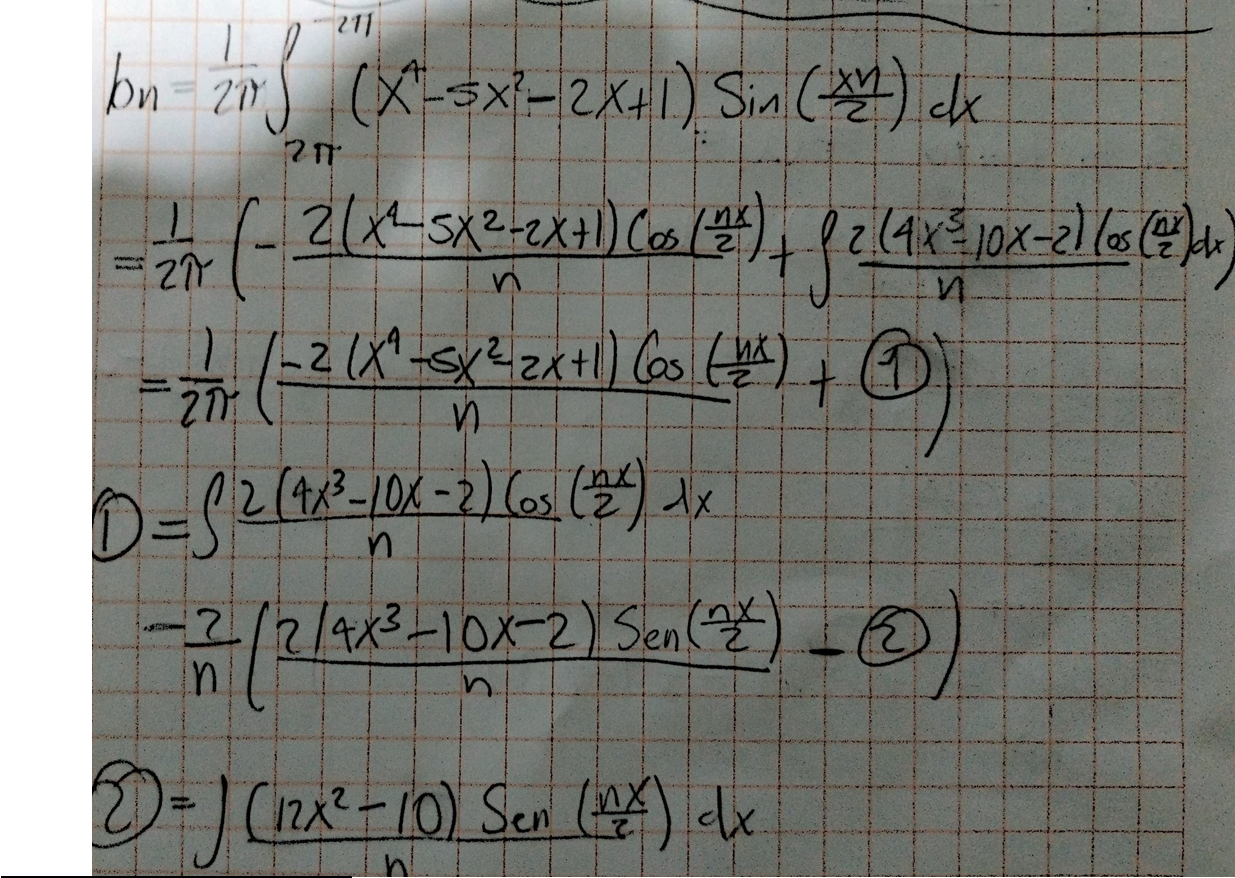
\includegraphics[width=4.74479in,height=3.37337in]{media/image47.png}

Imagen 7A. Procedimiento de Fourier

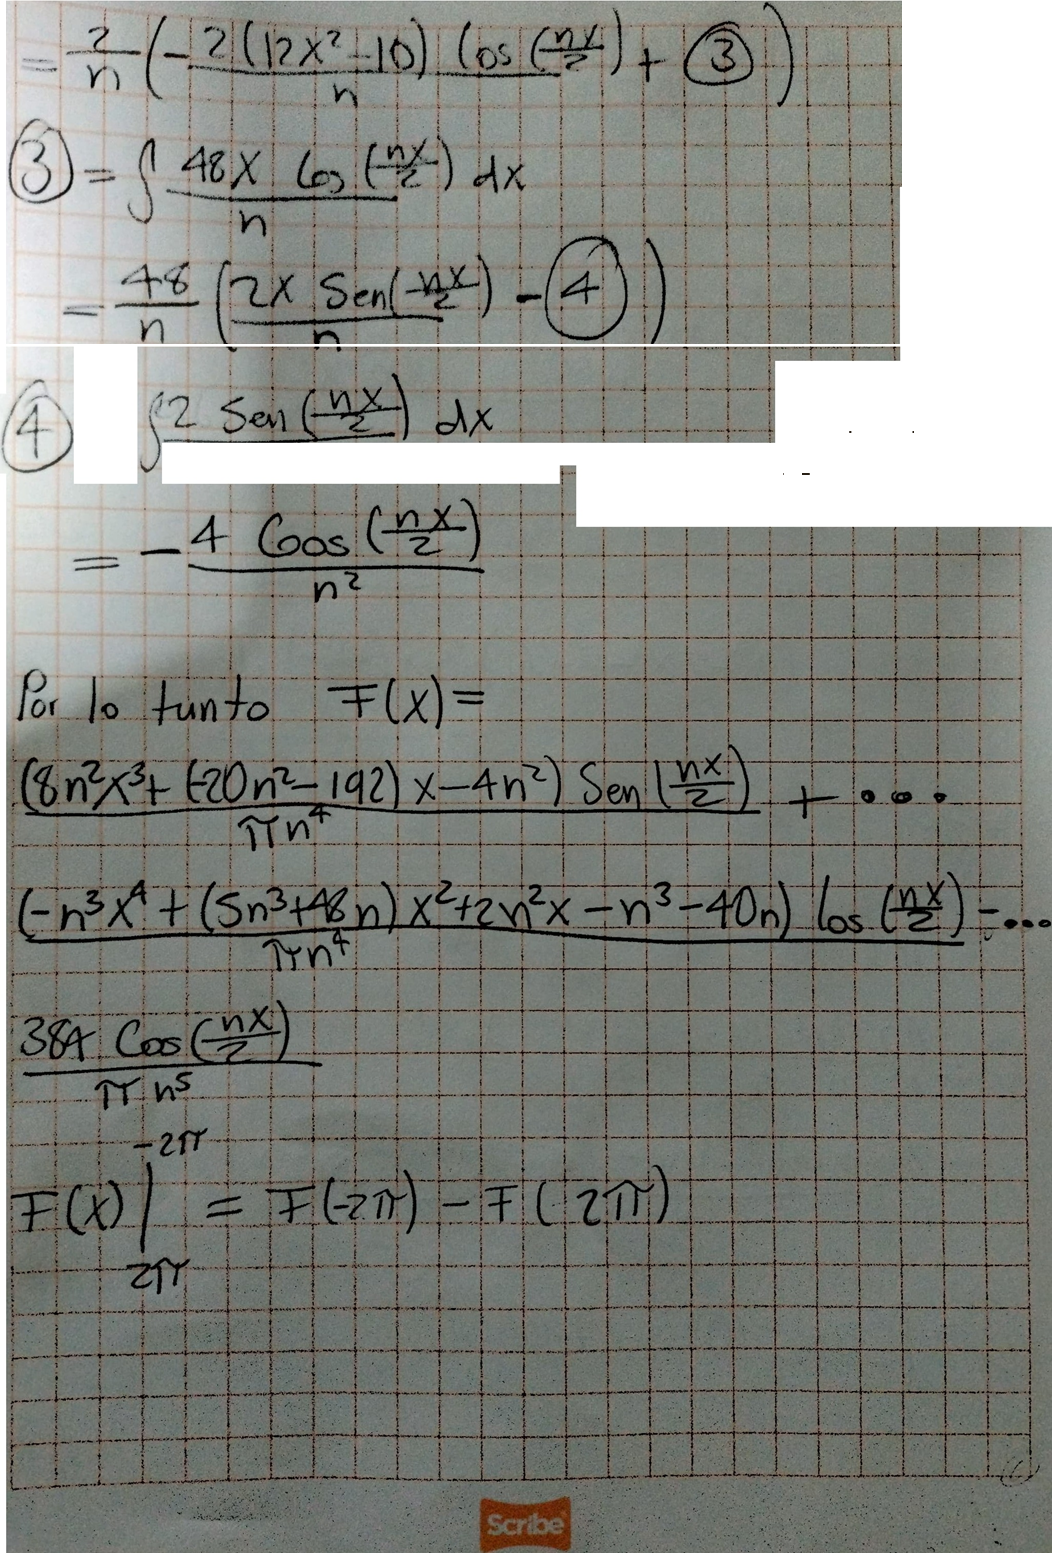
\includegraphics[width=4.94271in,height=7.29091in]{media/image53.png}

Imagen 8A. Procedimiento de Fourier

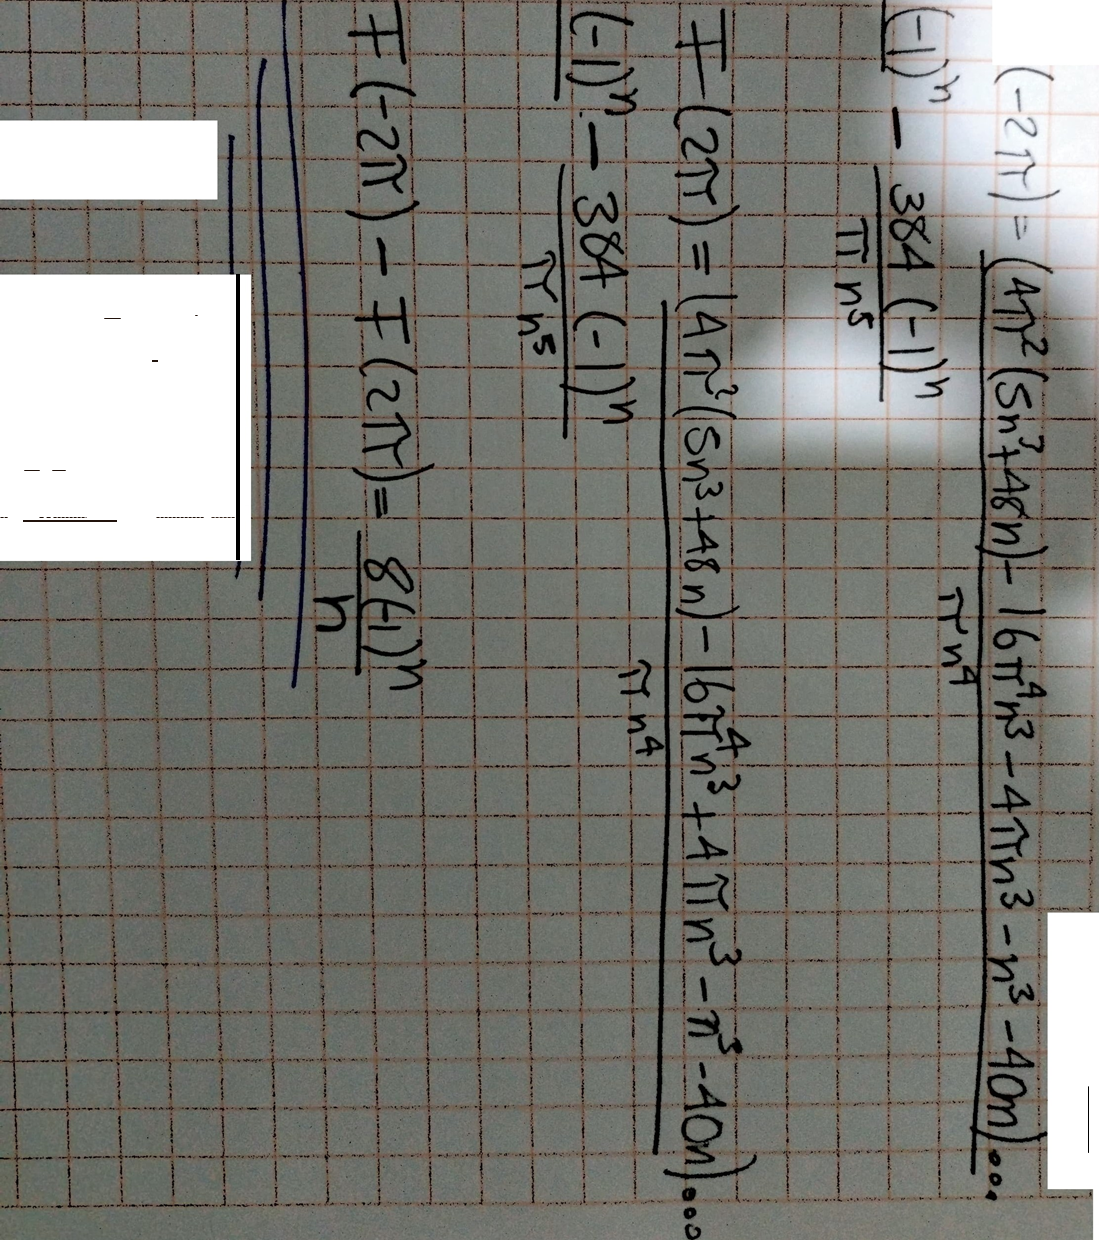
\includegraphics[width=3.88021in,height=4.37099in]{media/image43.png}

Imagen 9A. Procedimiento de Fourier

\subsection{\texorpdfstring{Magaly Citlali Jimeno Reyes }{Magaly Citlali Jimeno Reyes }}\label{magaly-citlali-jimeno-reyes}

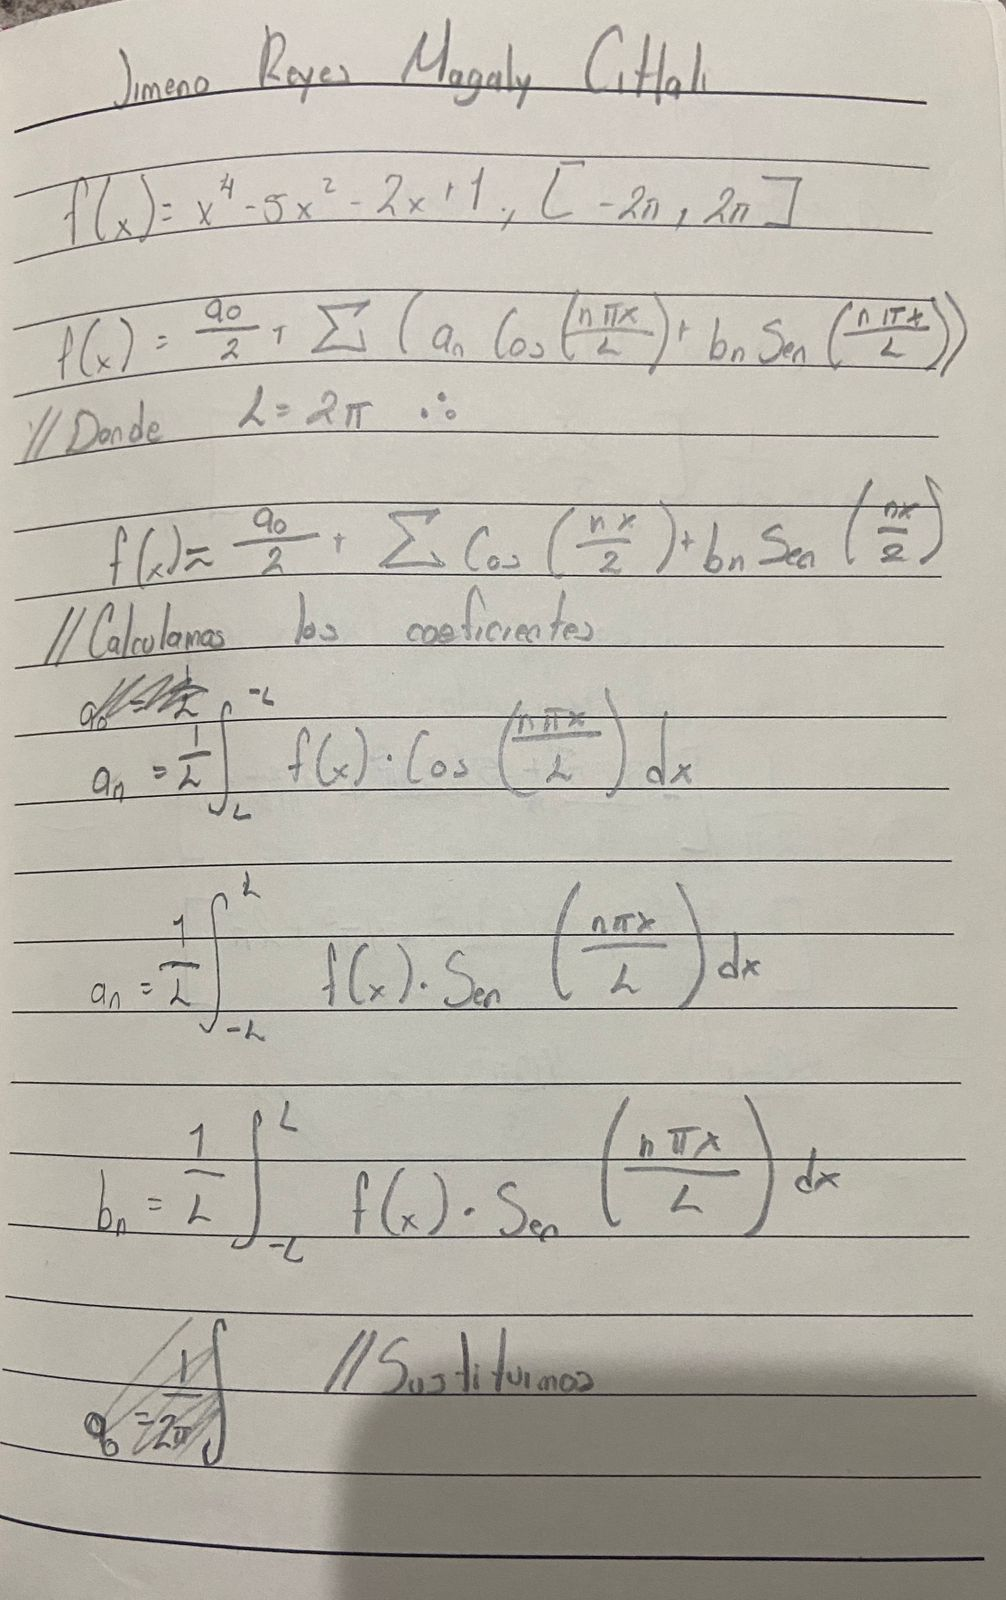
\includegraphics[width=2.98958in,height=4.74434in]{media/image13.jpg}

Imagen 1B. Procedimiento de Fourier

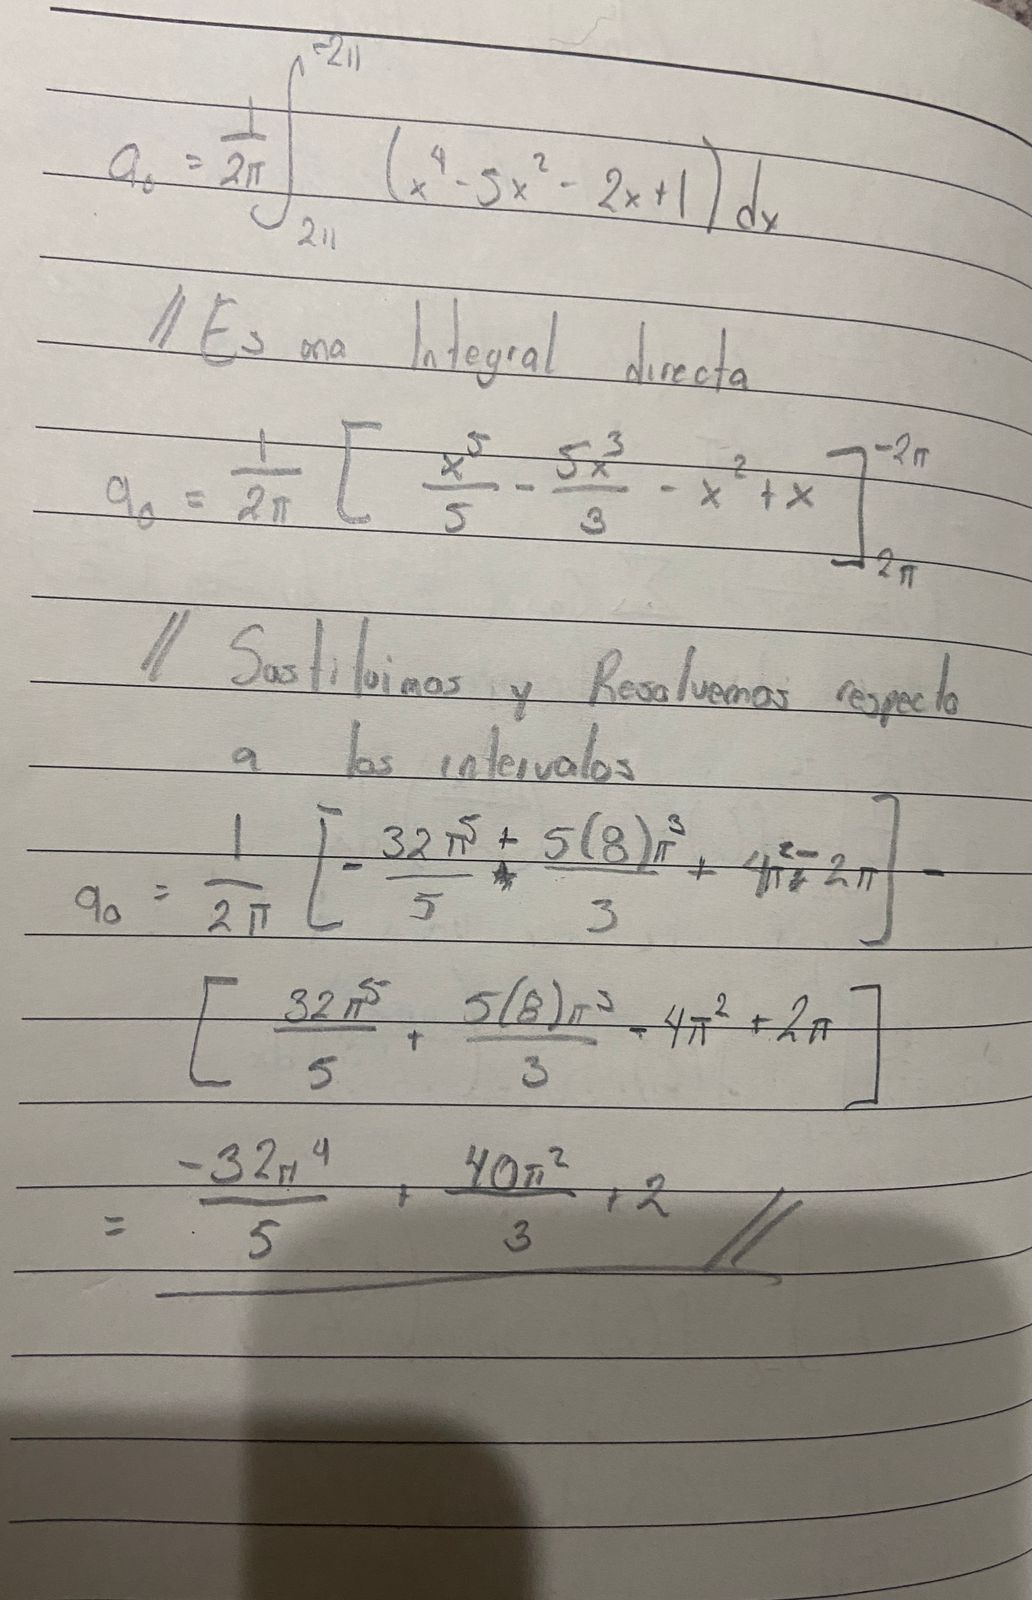
\includegraphics[width=3.03622in,height=4.74409in]{media/image8.jpg}

Imagen 2B. Procedimiento de Fourier

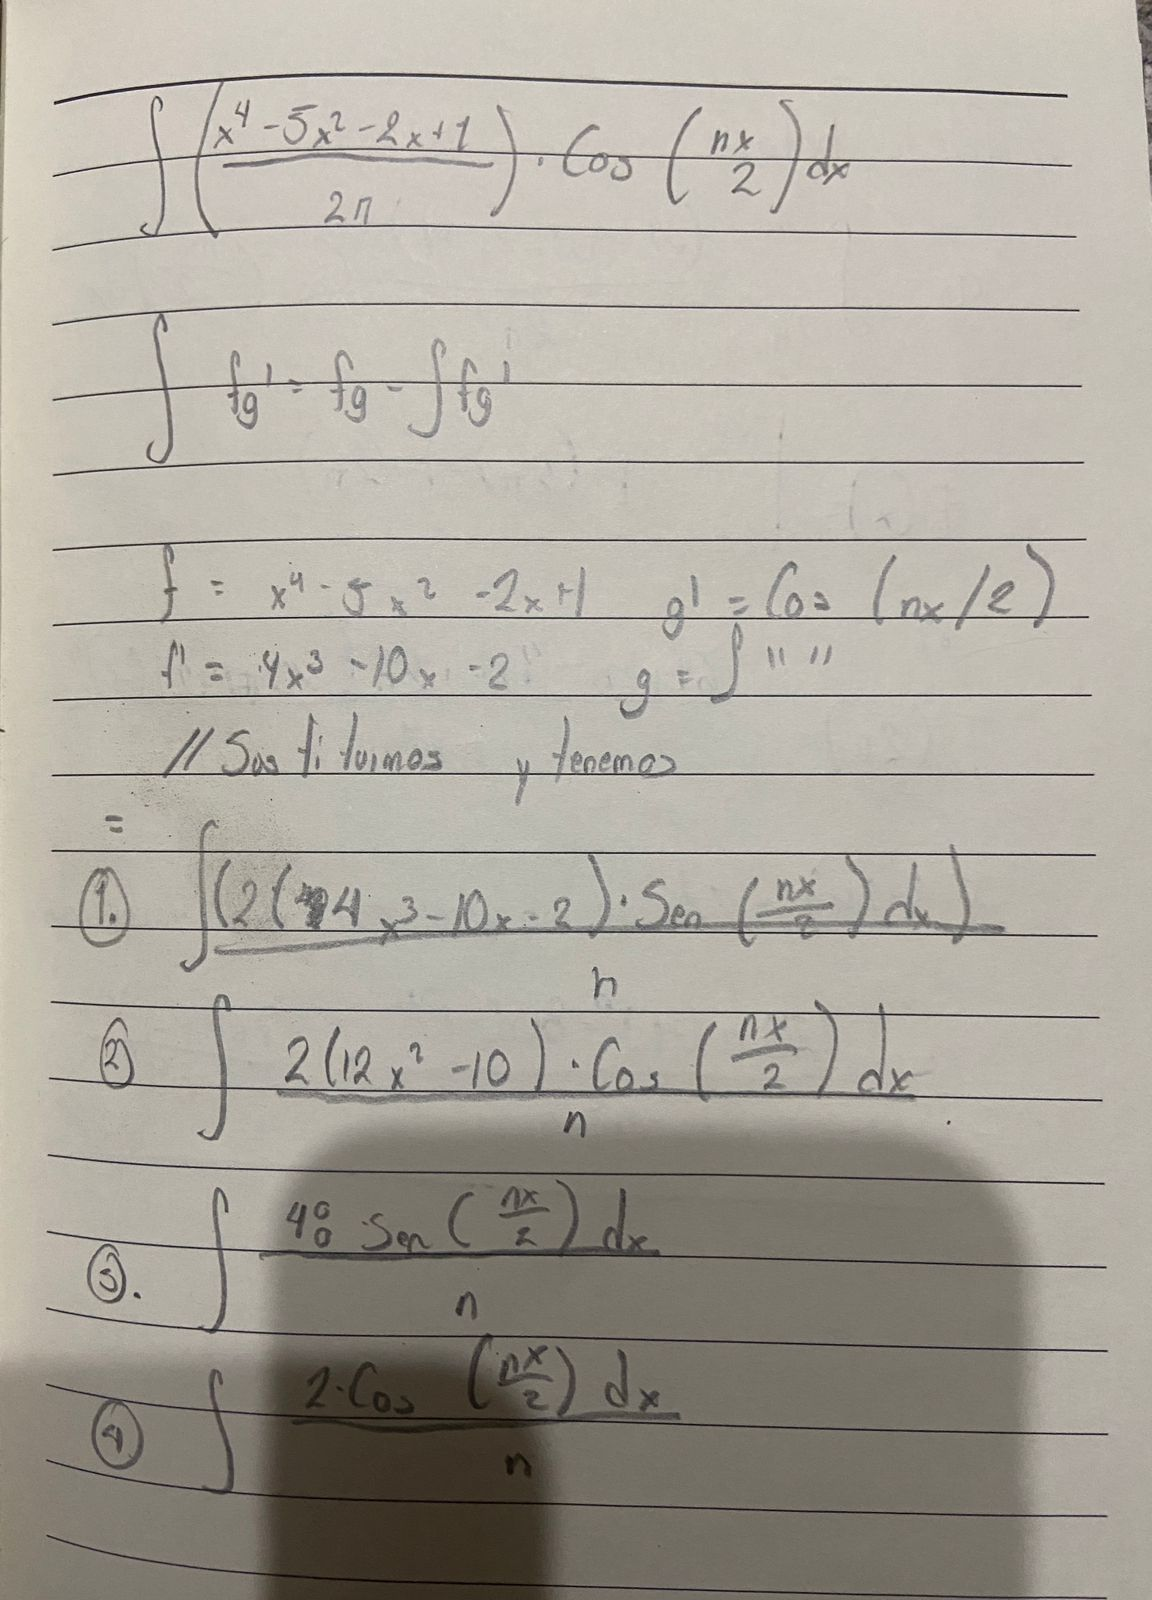
\includegraphics[width=3.0625in,height=5.18146in]{media/image42.jpg}

Imagen 3B. Procedimiento de Fourier

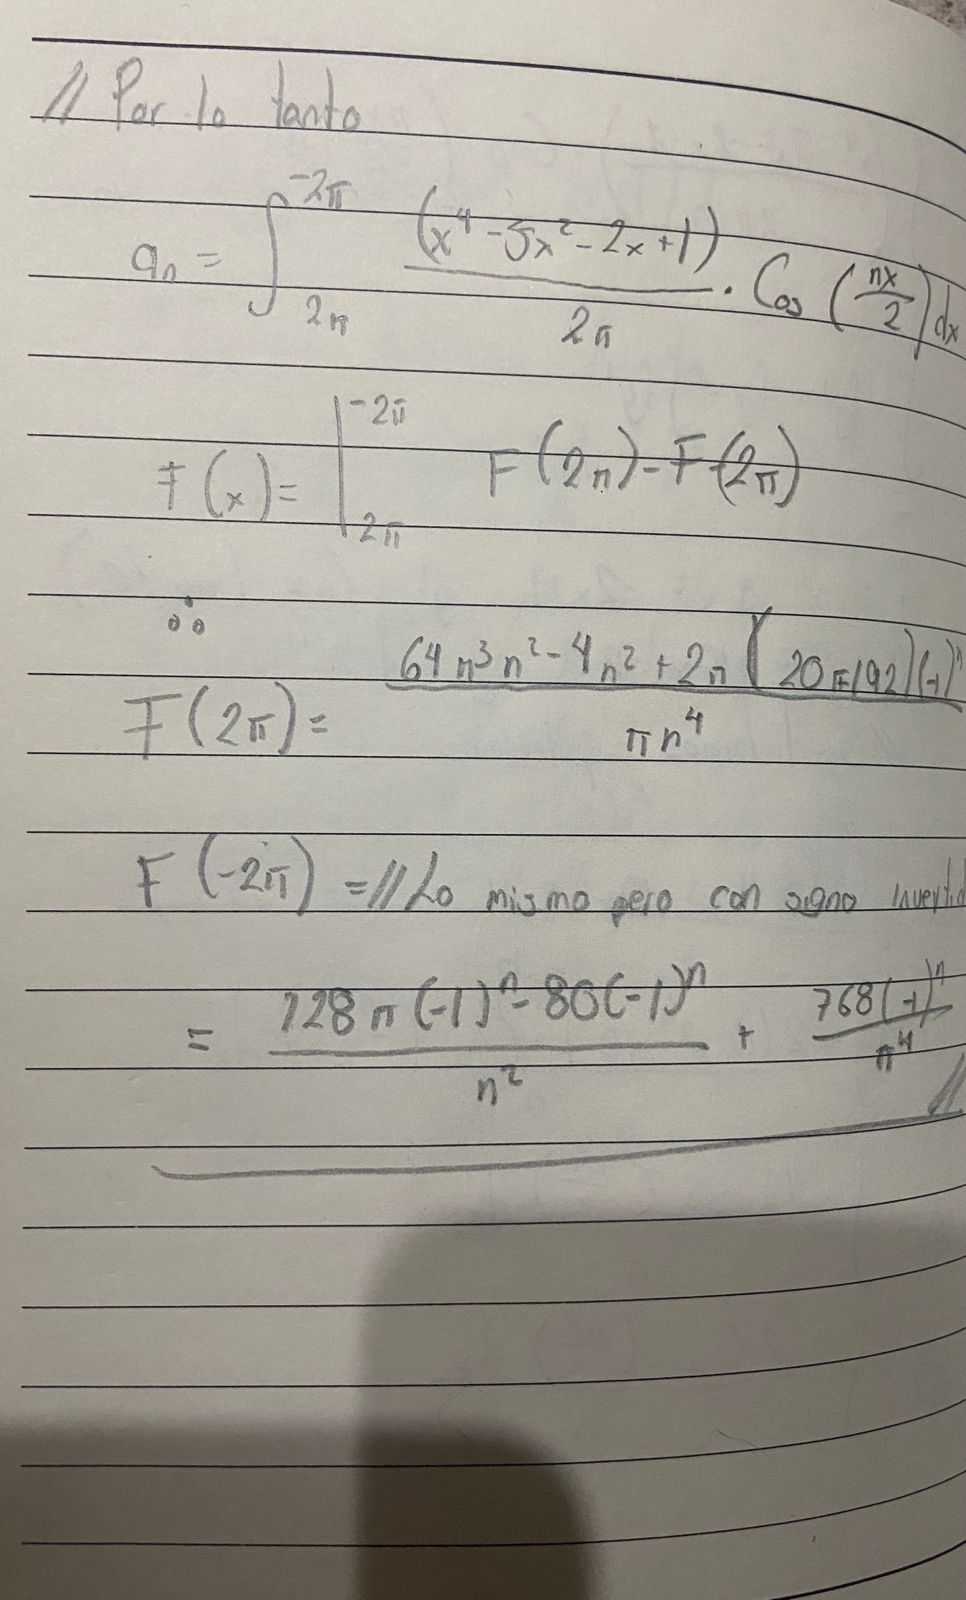
\includegraphics[width=2.97297in,height=4.92052in]{media/image2.jpg}

Imagen 4B. Procedimiento de Fourier

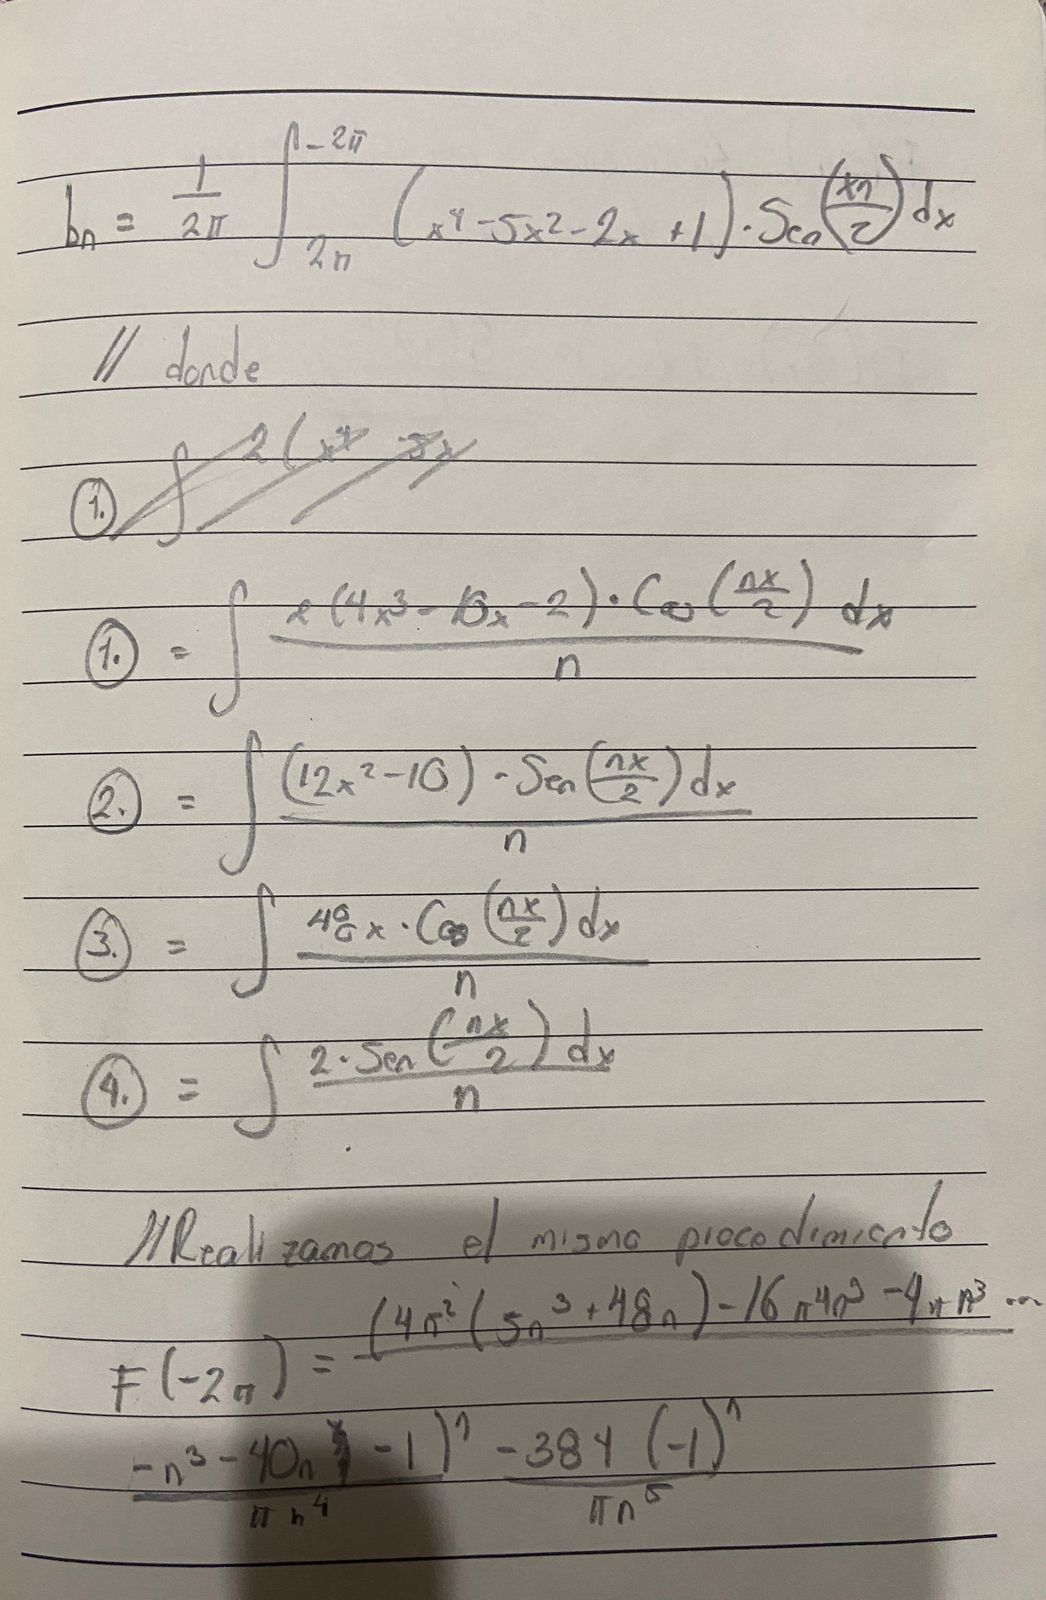
\includegraphics[width=3.1436in,height=4.80787in]{media/image9.jpg}

Imagen 5B. Procedimiento de Fourier

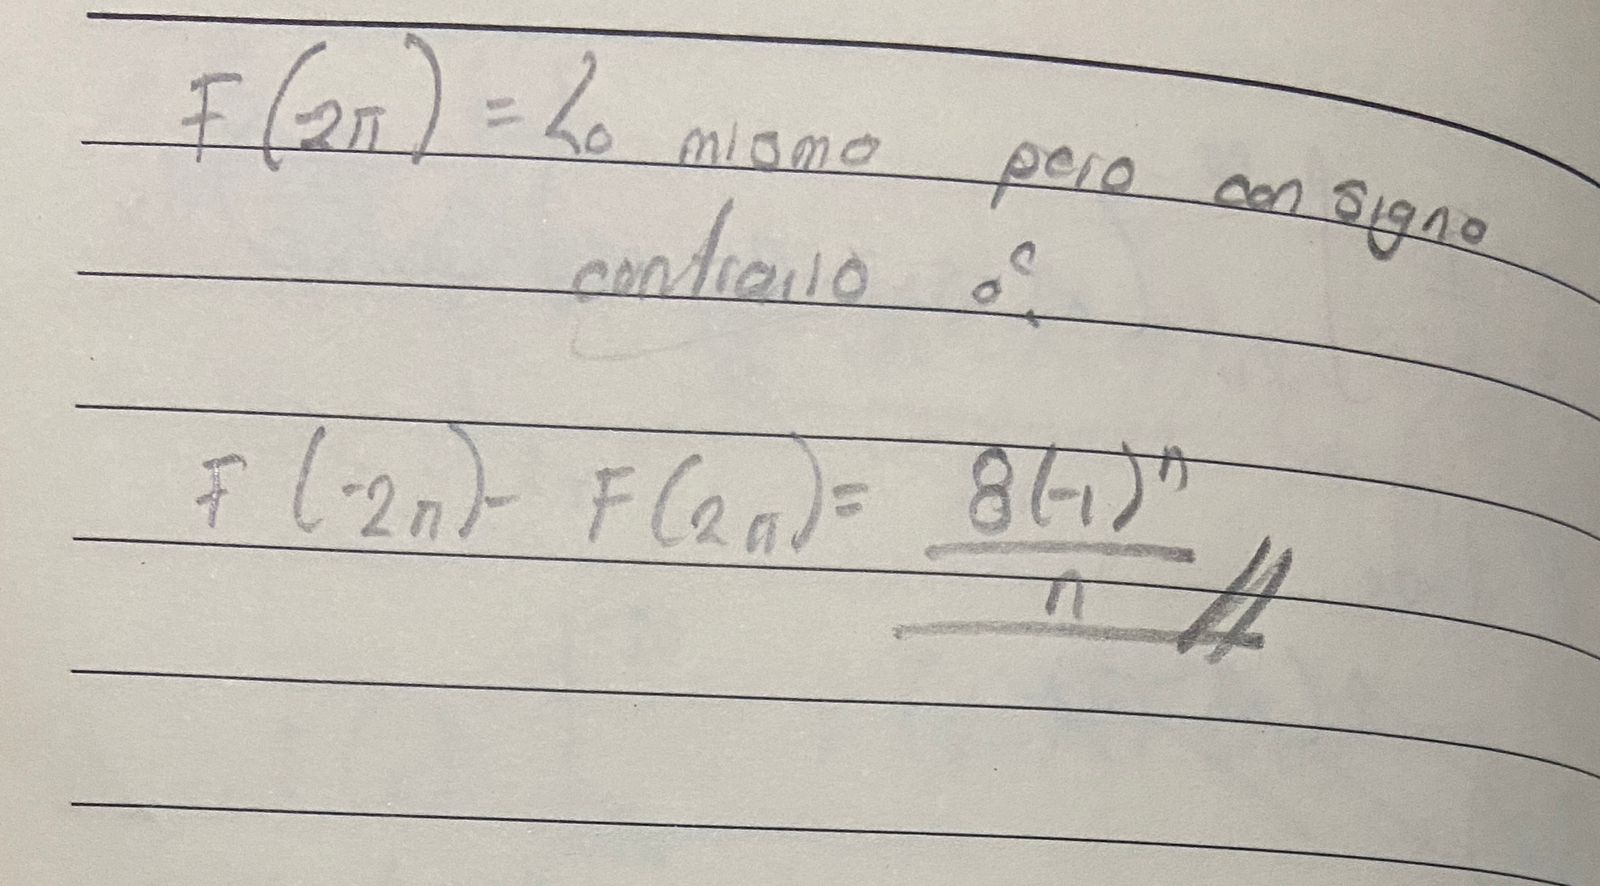
\includegraphics[width=3.00684in,height=3.1593in]{media/image46.jpg}

Imagen 6B. Procedimiento de Fourier

\subsection{Juárez Botello Josué Adalid}\label{juuxe1rez-botello-josuuxe9-adalid}

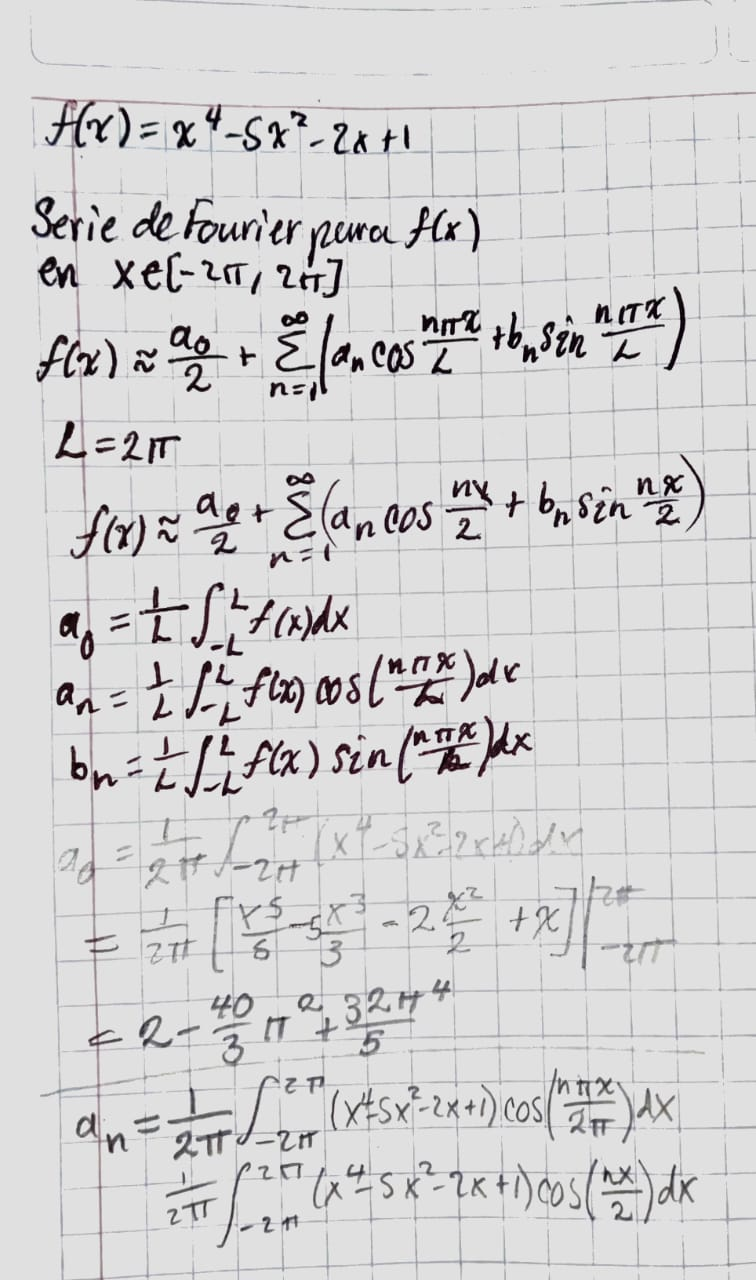
\includegraphics[width=3.19696in,height=5.41146in]{media/image44.jpg}\\ Imagen C1. Primero, establecemos la forma de la serie de la función f(x).

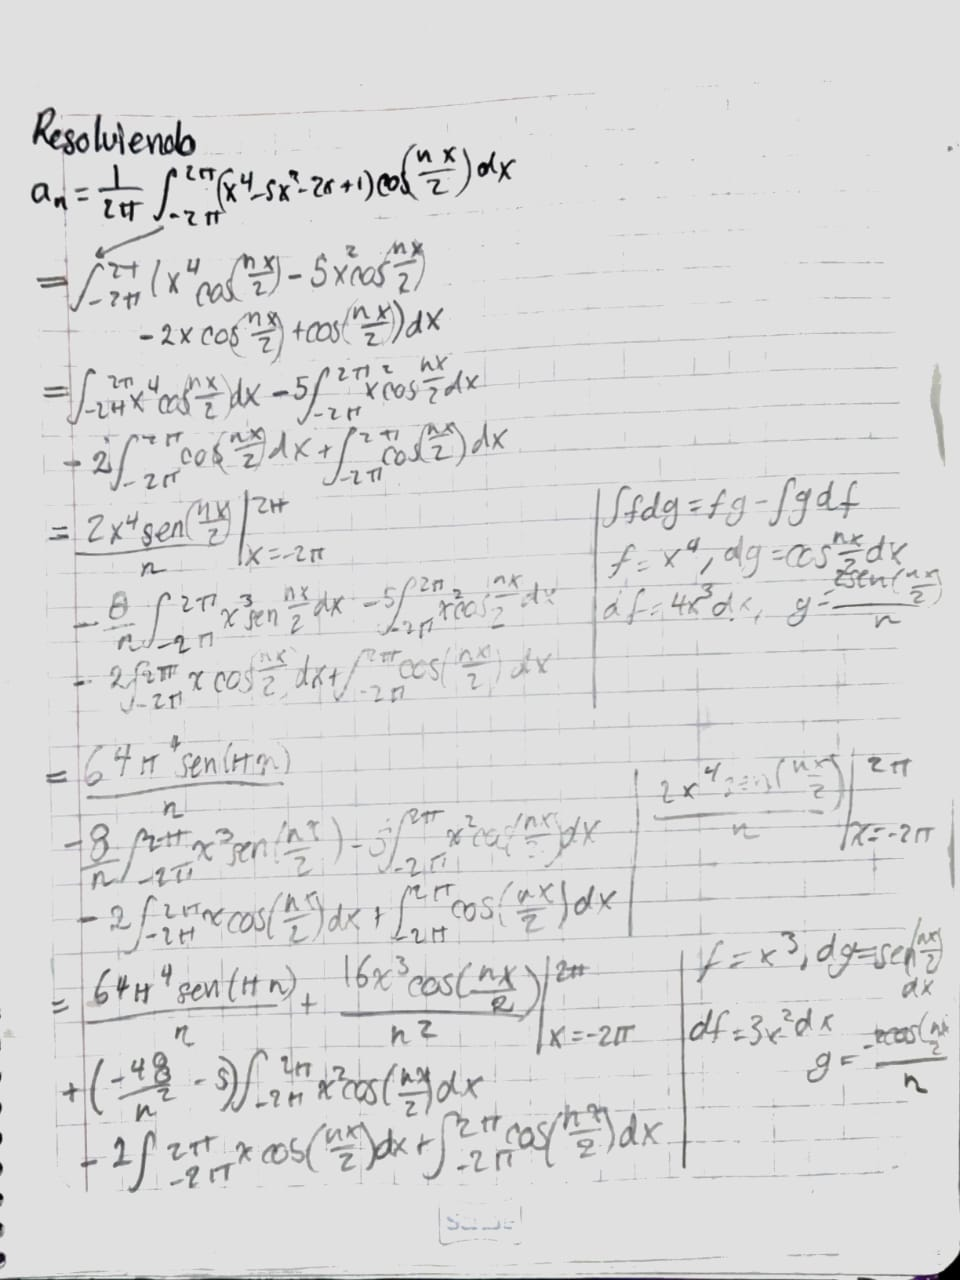
\includegraphics[width=3.12761in,height=4.17188in]{media/image31.jpg}\\ Imagen C2. Primero determinaremos la forma cerrada del término a\_n.

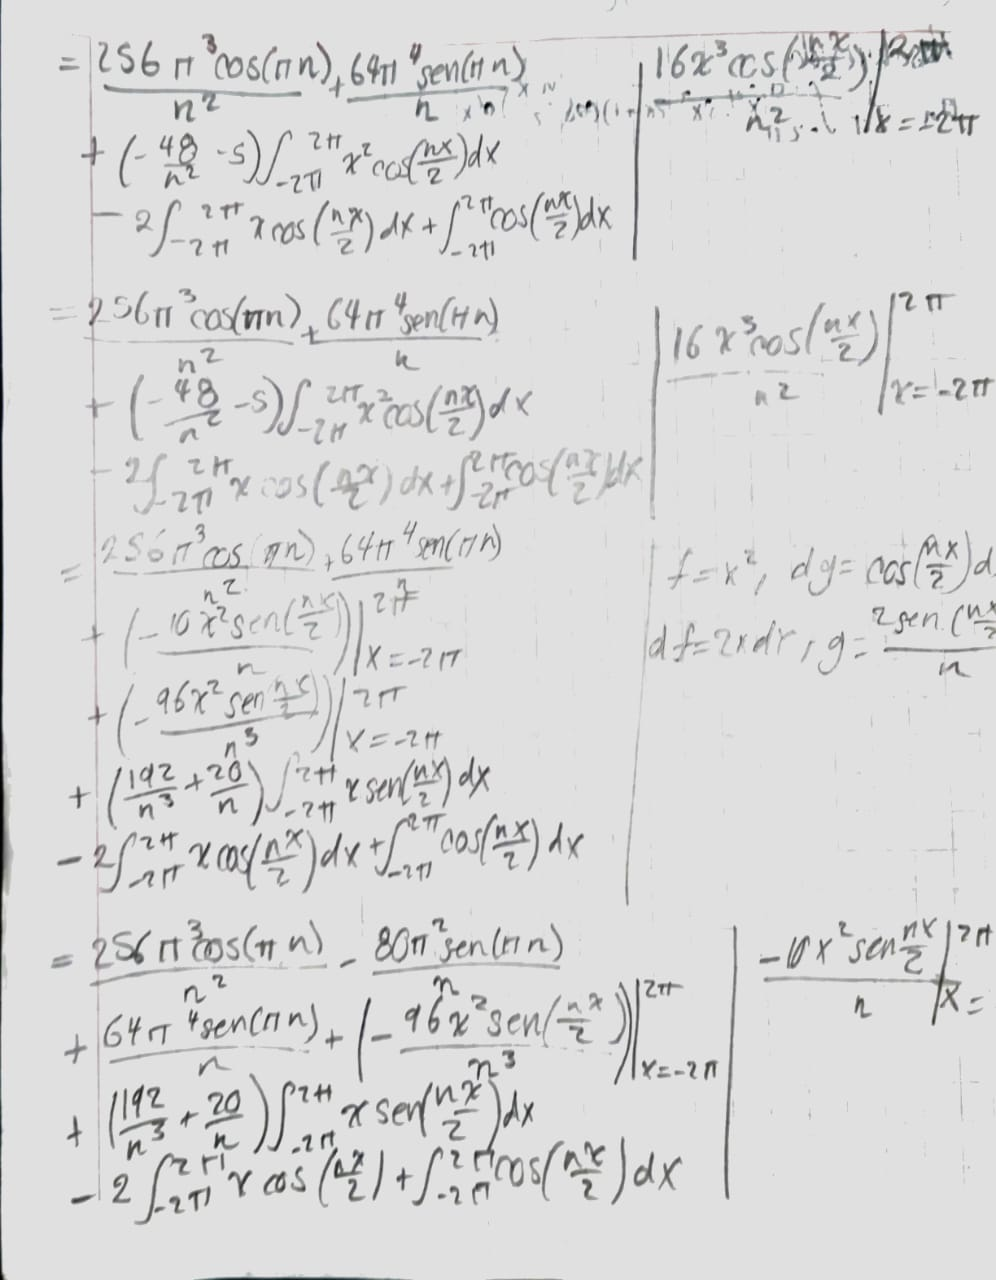
\includegraphics[width=2.78659in,height=3.57813in]{media/image34.jpg}

Imagen C3. continuación del cálculo a\_n.

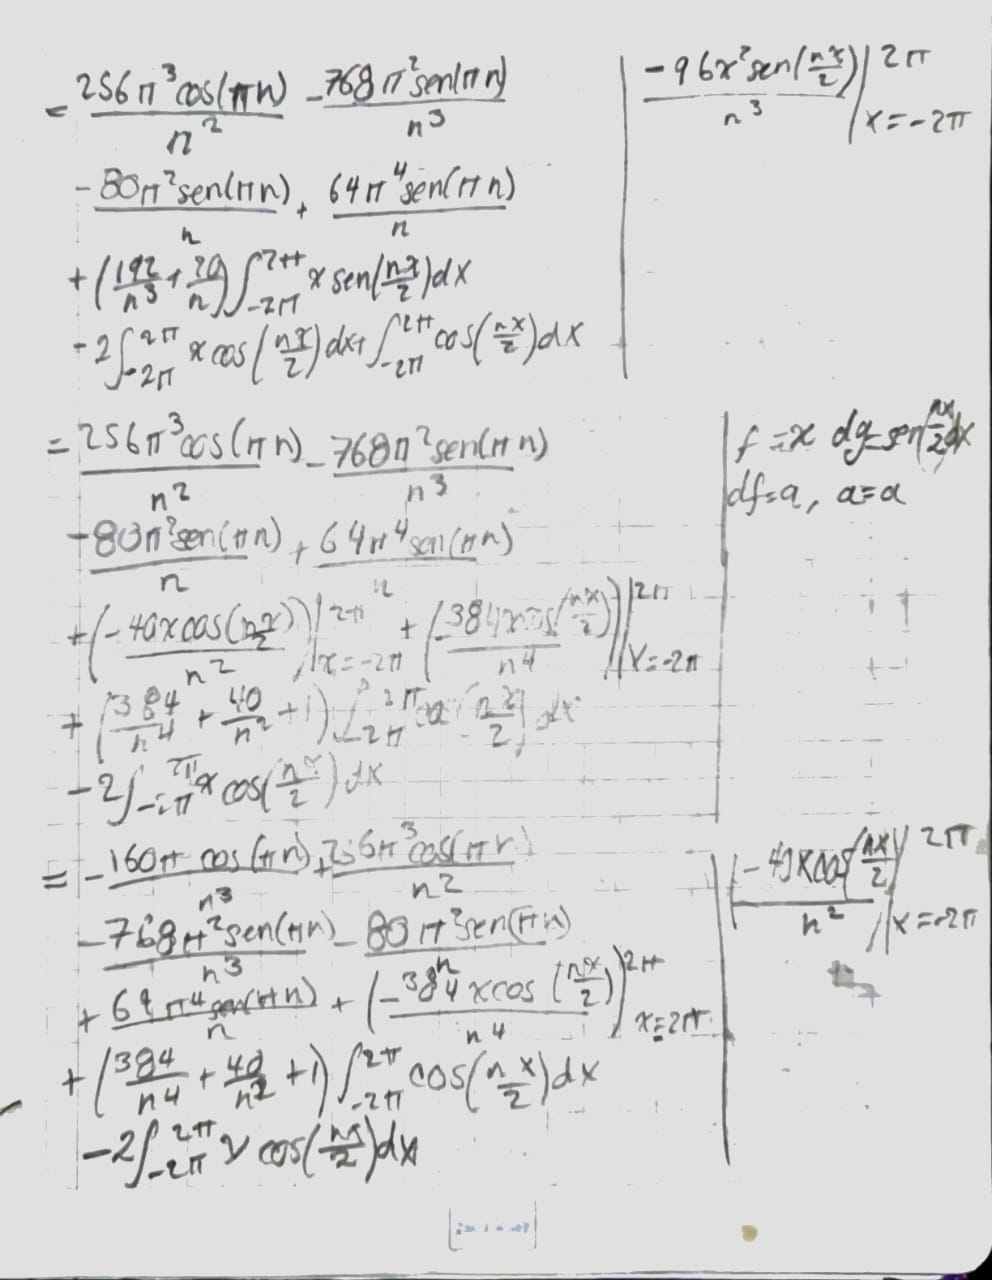
\includegraphics[width=2.84046in,height=3.66146in]{media/image14.jpg}\\ Imagen C4. Continuación cálculo a\_n.

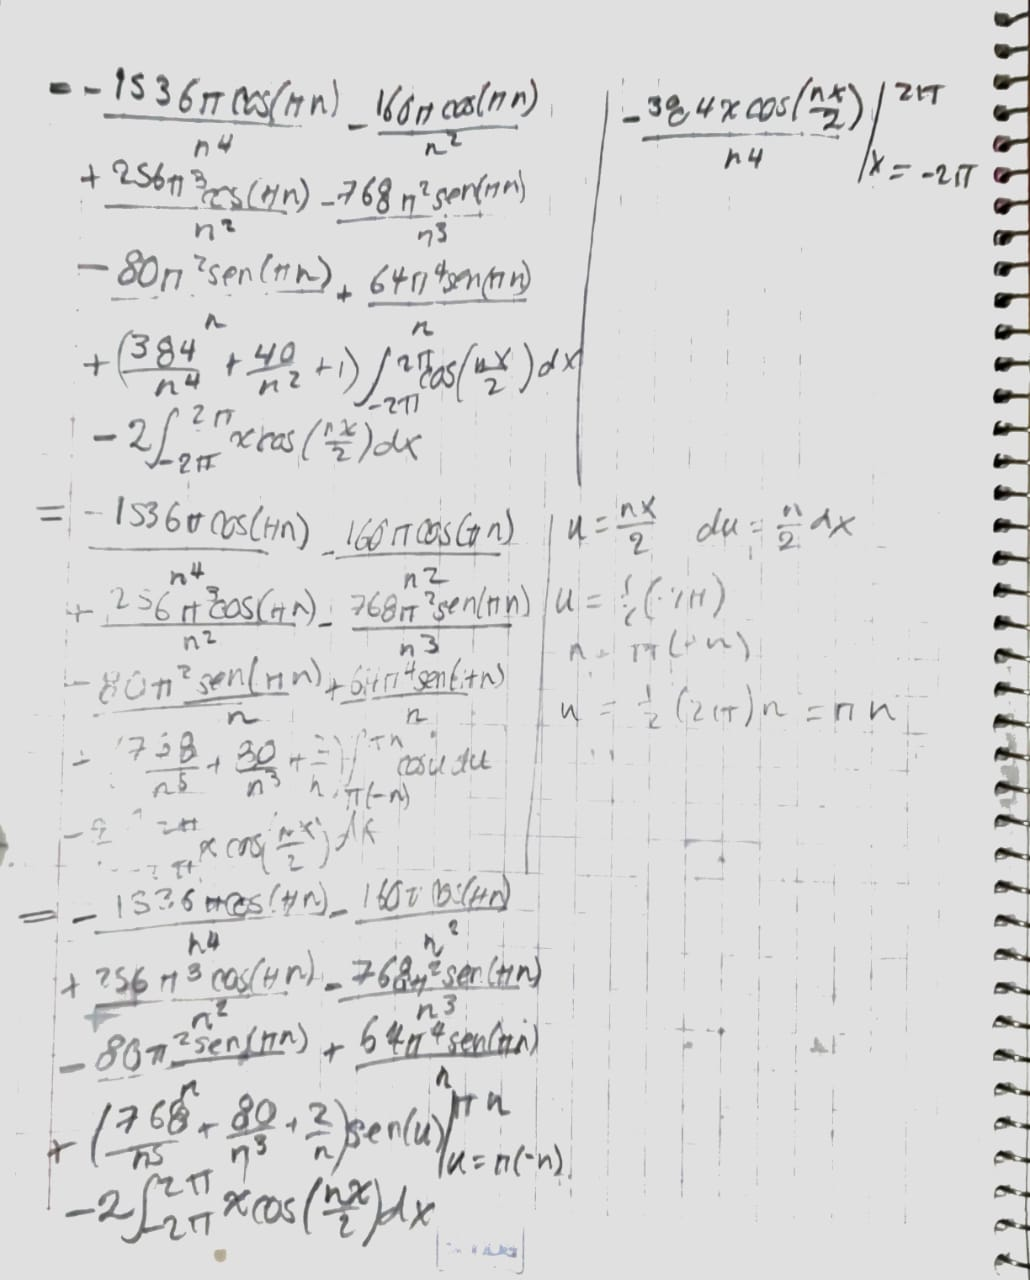
\includegraphics[width=2.66175in,height=3.30729in]{media/image15.jpg}

Imagen C5. Continuación cálculo a\_n.

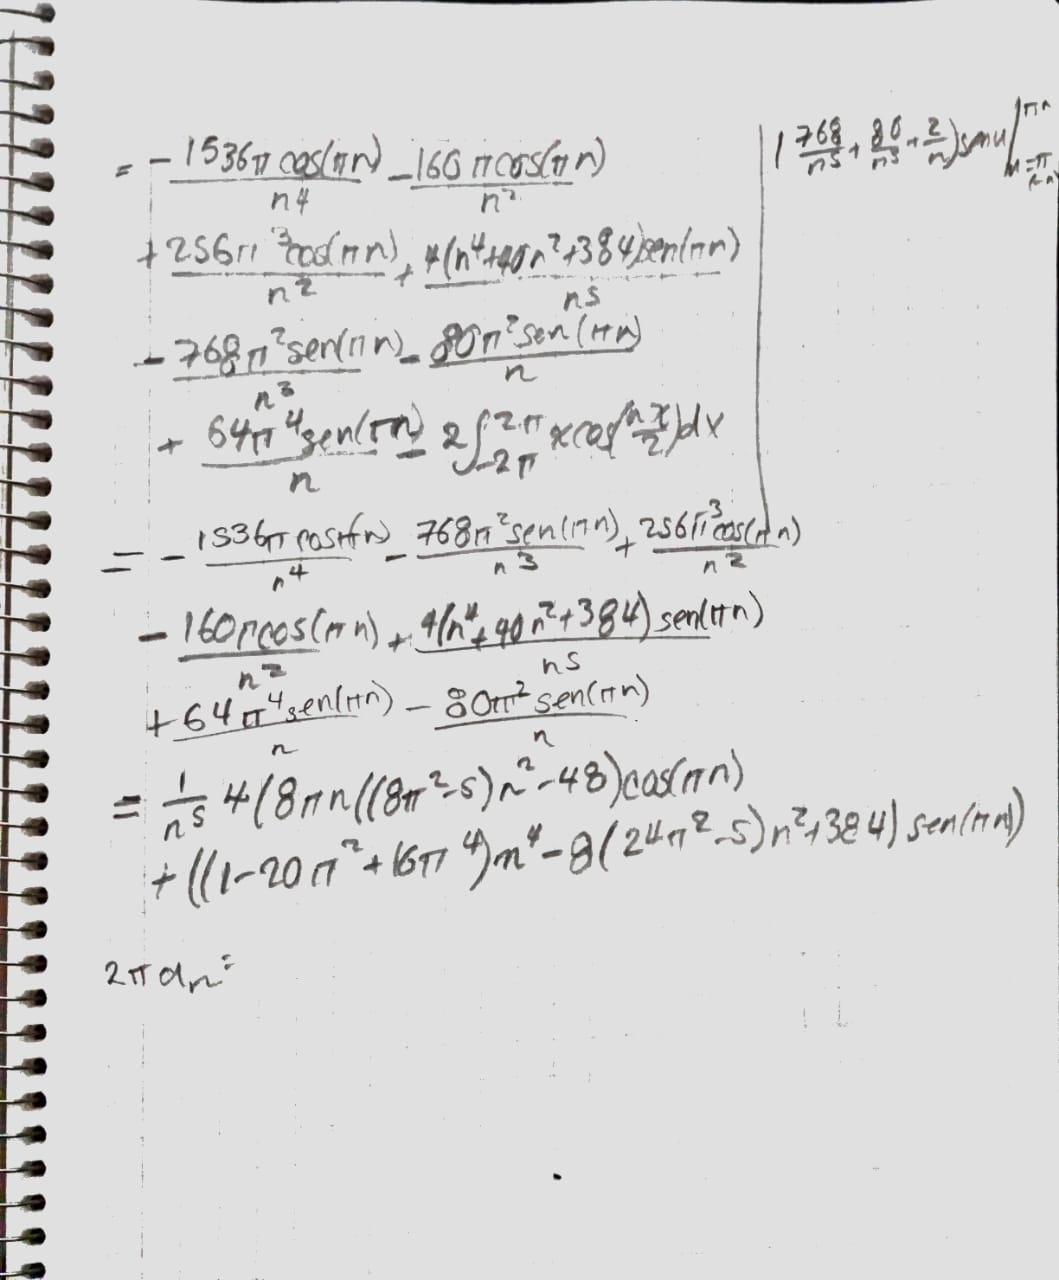
\includegraphics[width=3.09896in,height=3.74243in]{media/image45.jpg}\\ Imagen C6. Finalmente, definimos que el término a\_n es igual a lo que se muestra en la foto.

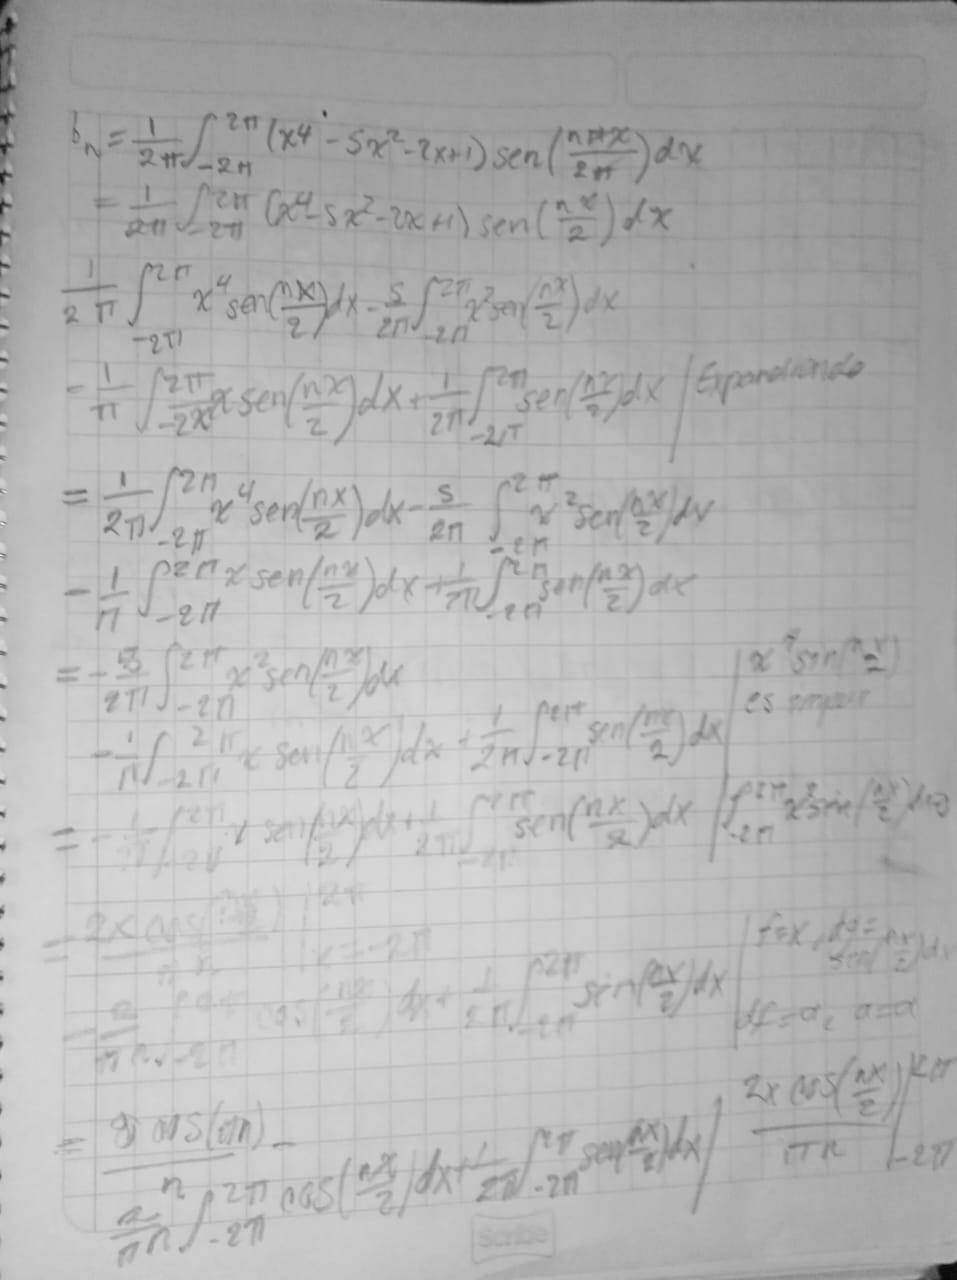
\includegraphics[width=2.6836in,height=3.58854in]{media/image26.jpg}\\ Imagen C7. Continuamos con la determinación del término b\_n

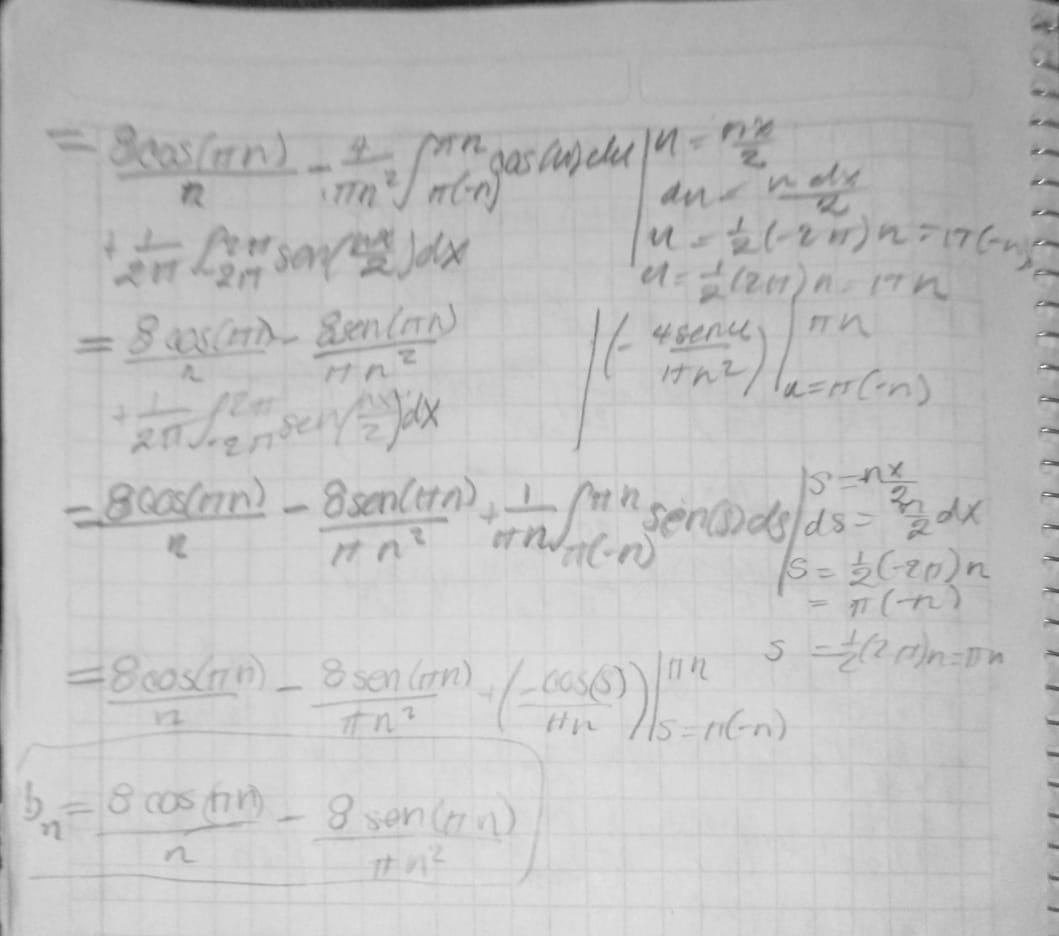
\includegraphics[width=4.00521in,height=3.53949in]{media/image41.jpg}\\ Imagen C8. Y ese es el término b\_n para la serie de Fourier. Sustituímos en la forma de la serie mencionada al principio. Cabe señalar que fue mucho más sencillo calcular b\_n por la propiedad de la función seno de ser impar.

\subsection{Oscar Uriel Juarez Tolamatl}\label{oscar-uriel-juarez-tolamatl}

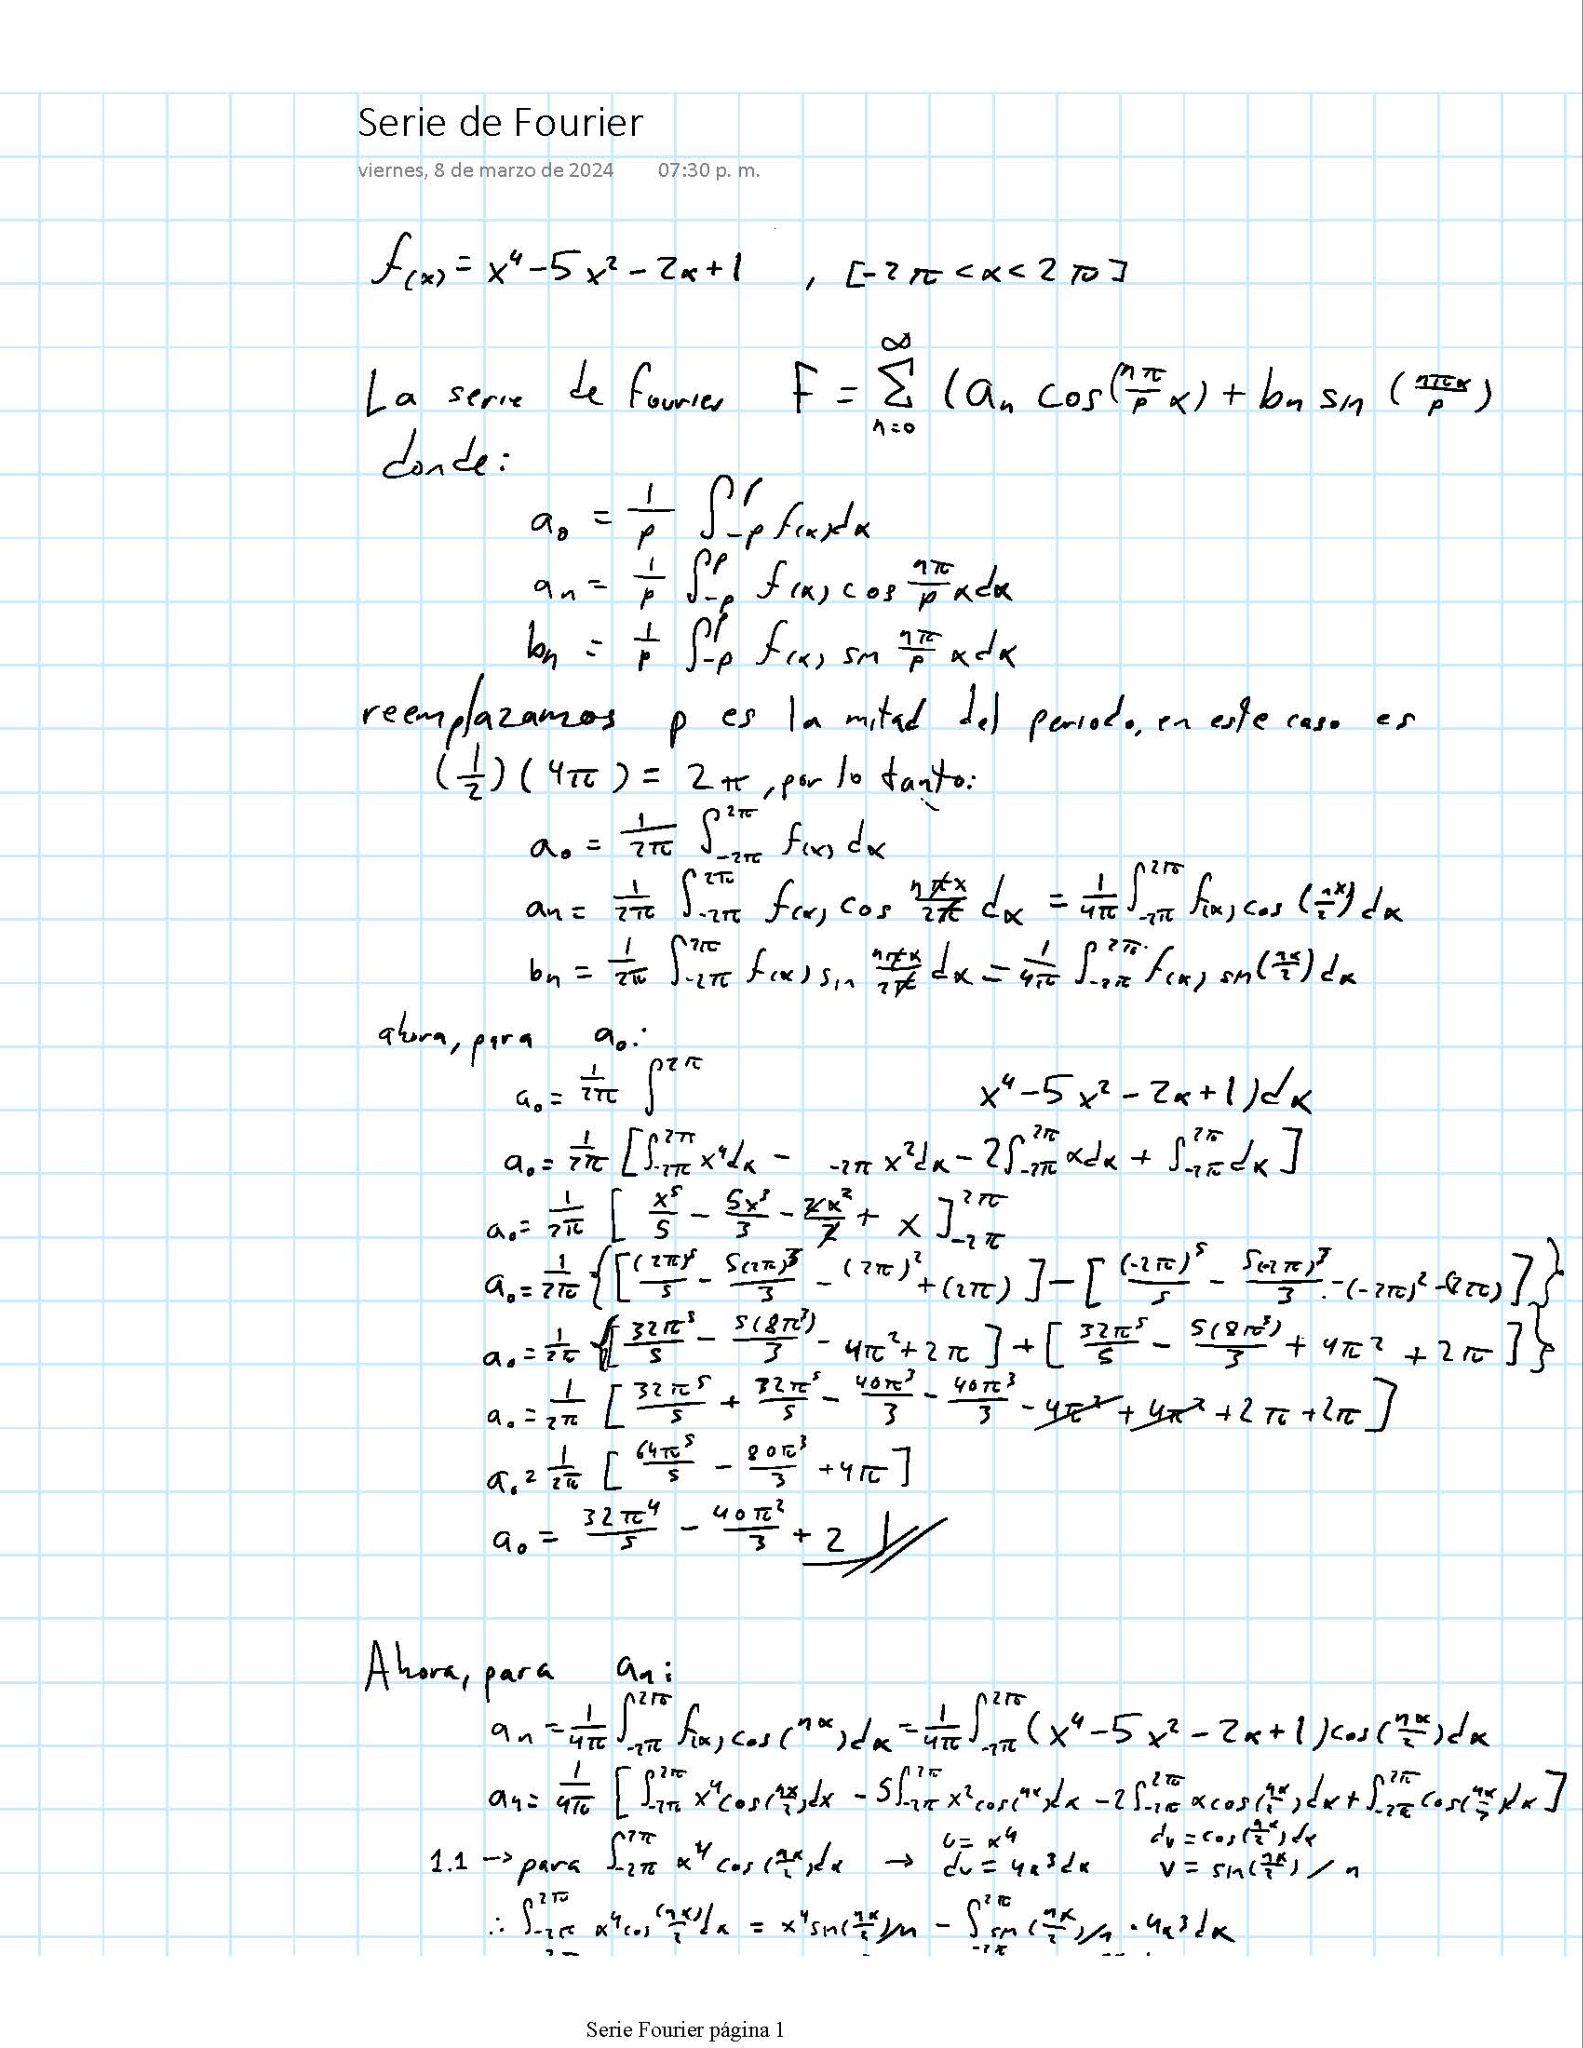
\includegraphics[width=5.93125in,height=7.67516in]{media/image59.jpg}

Imagen 1D. Procedimiento de Fourier

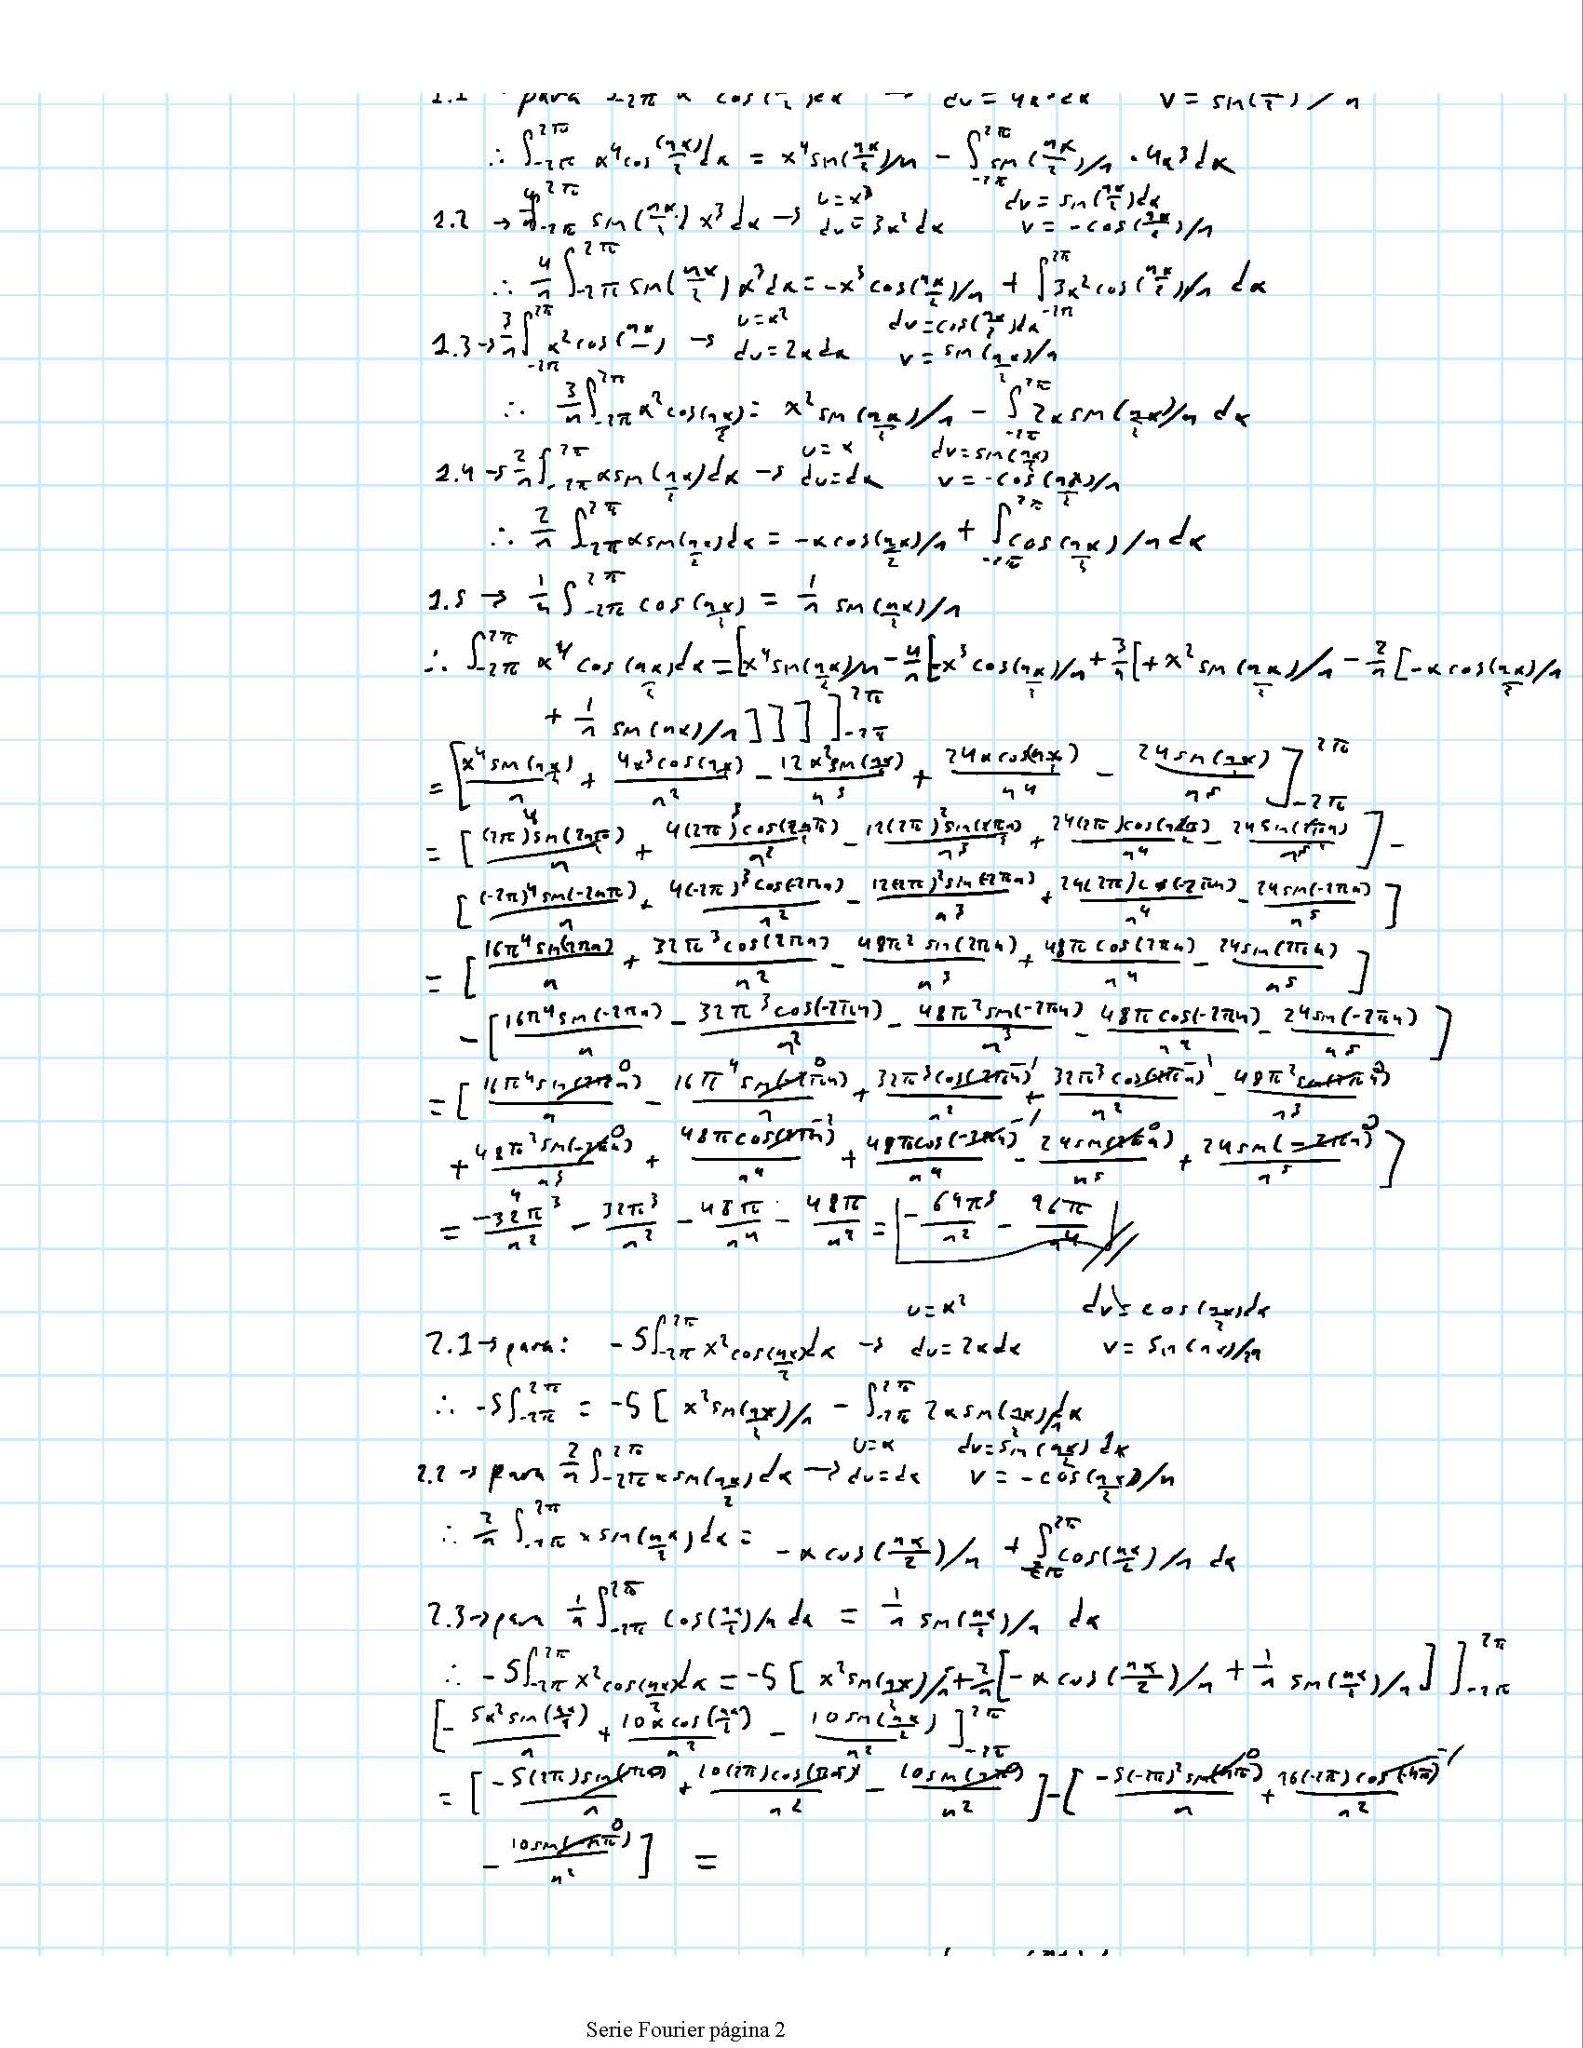
\includegraphics[width=6.26772in,height=8.11111in]{media/image56.jpg}

Imagen 2D. Procedimiento de Fourier

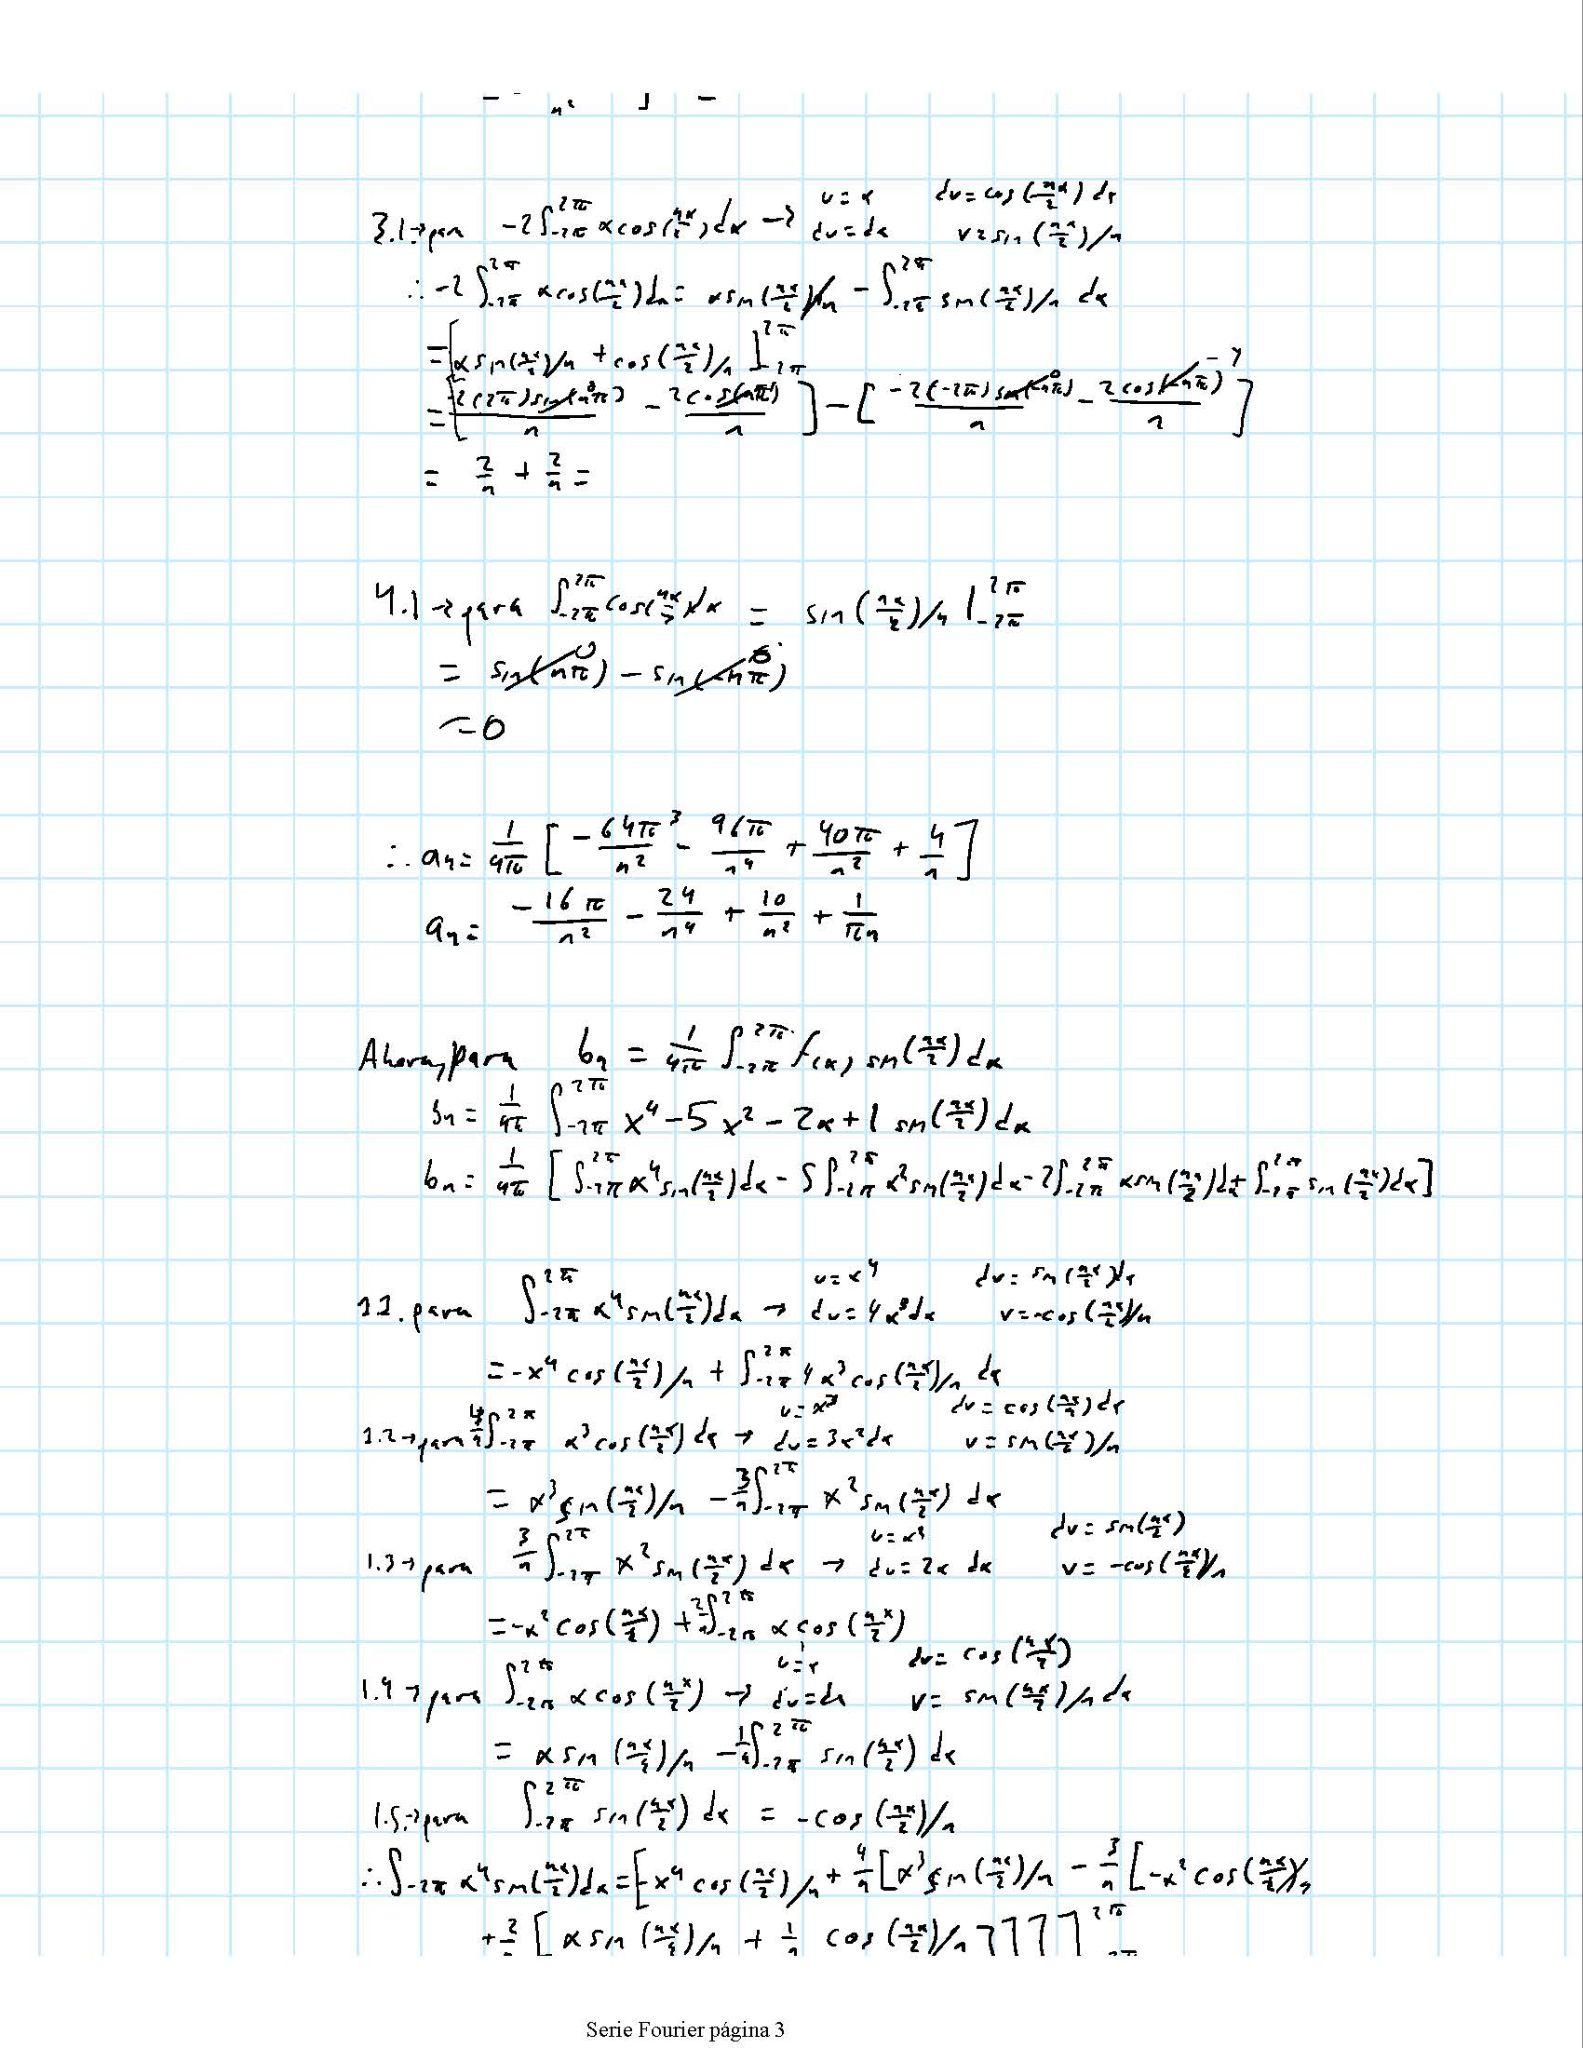
\includegraphics[width=6.26772in,height=8.11111in]{media/image55.jpg}

Imagen 3D. Procedimiento de Fourier

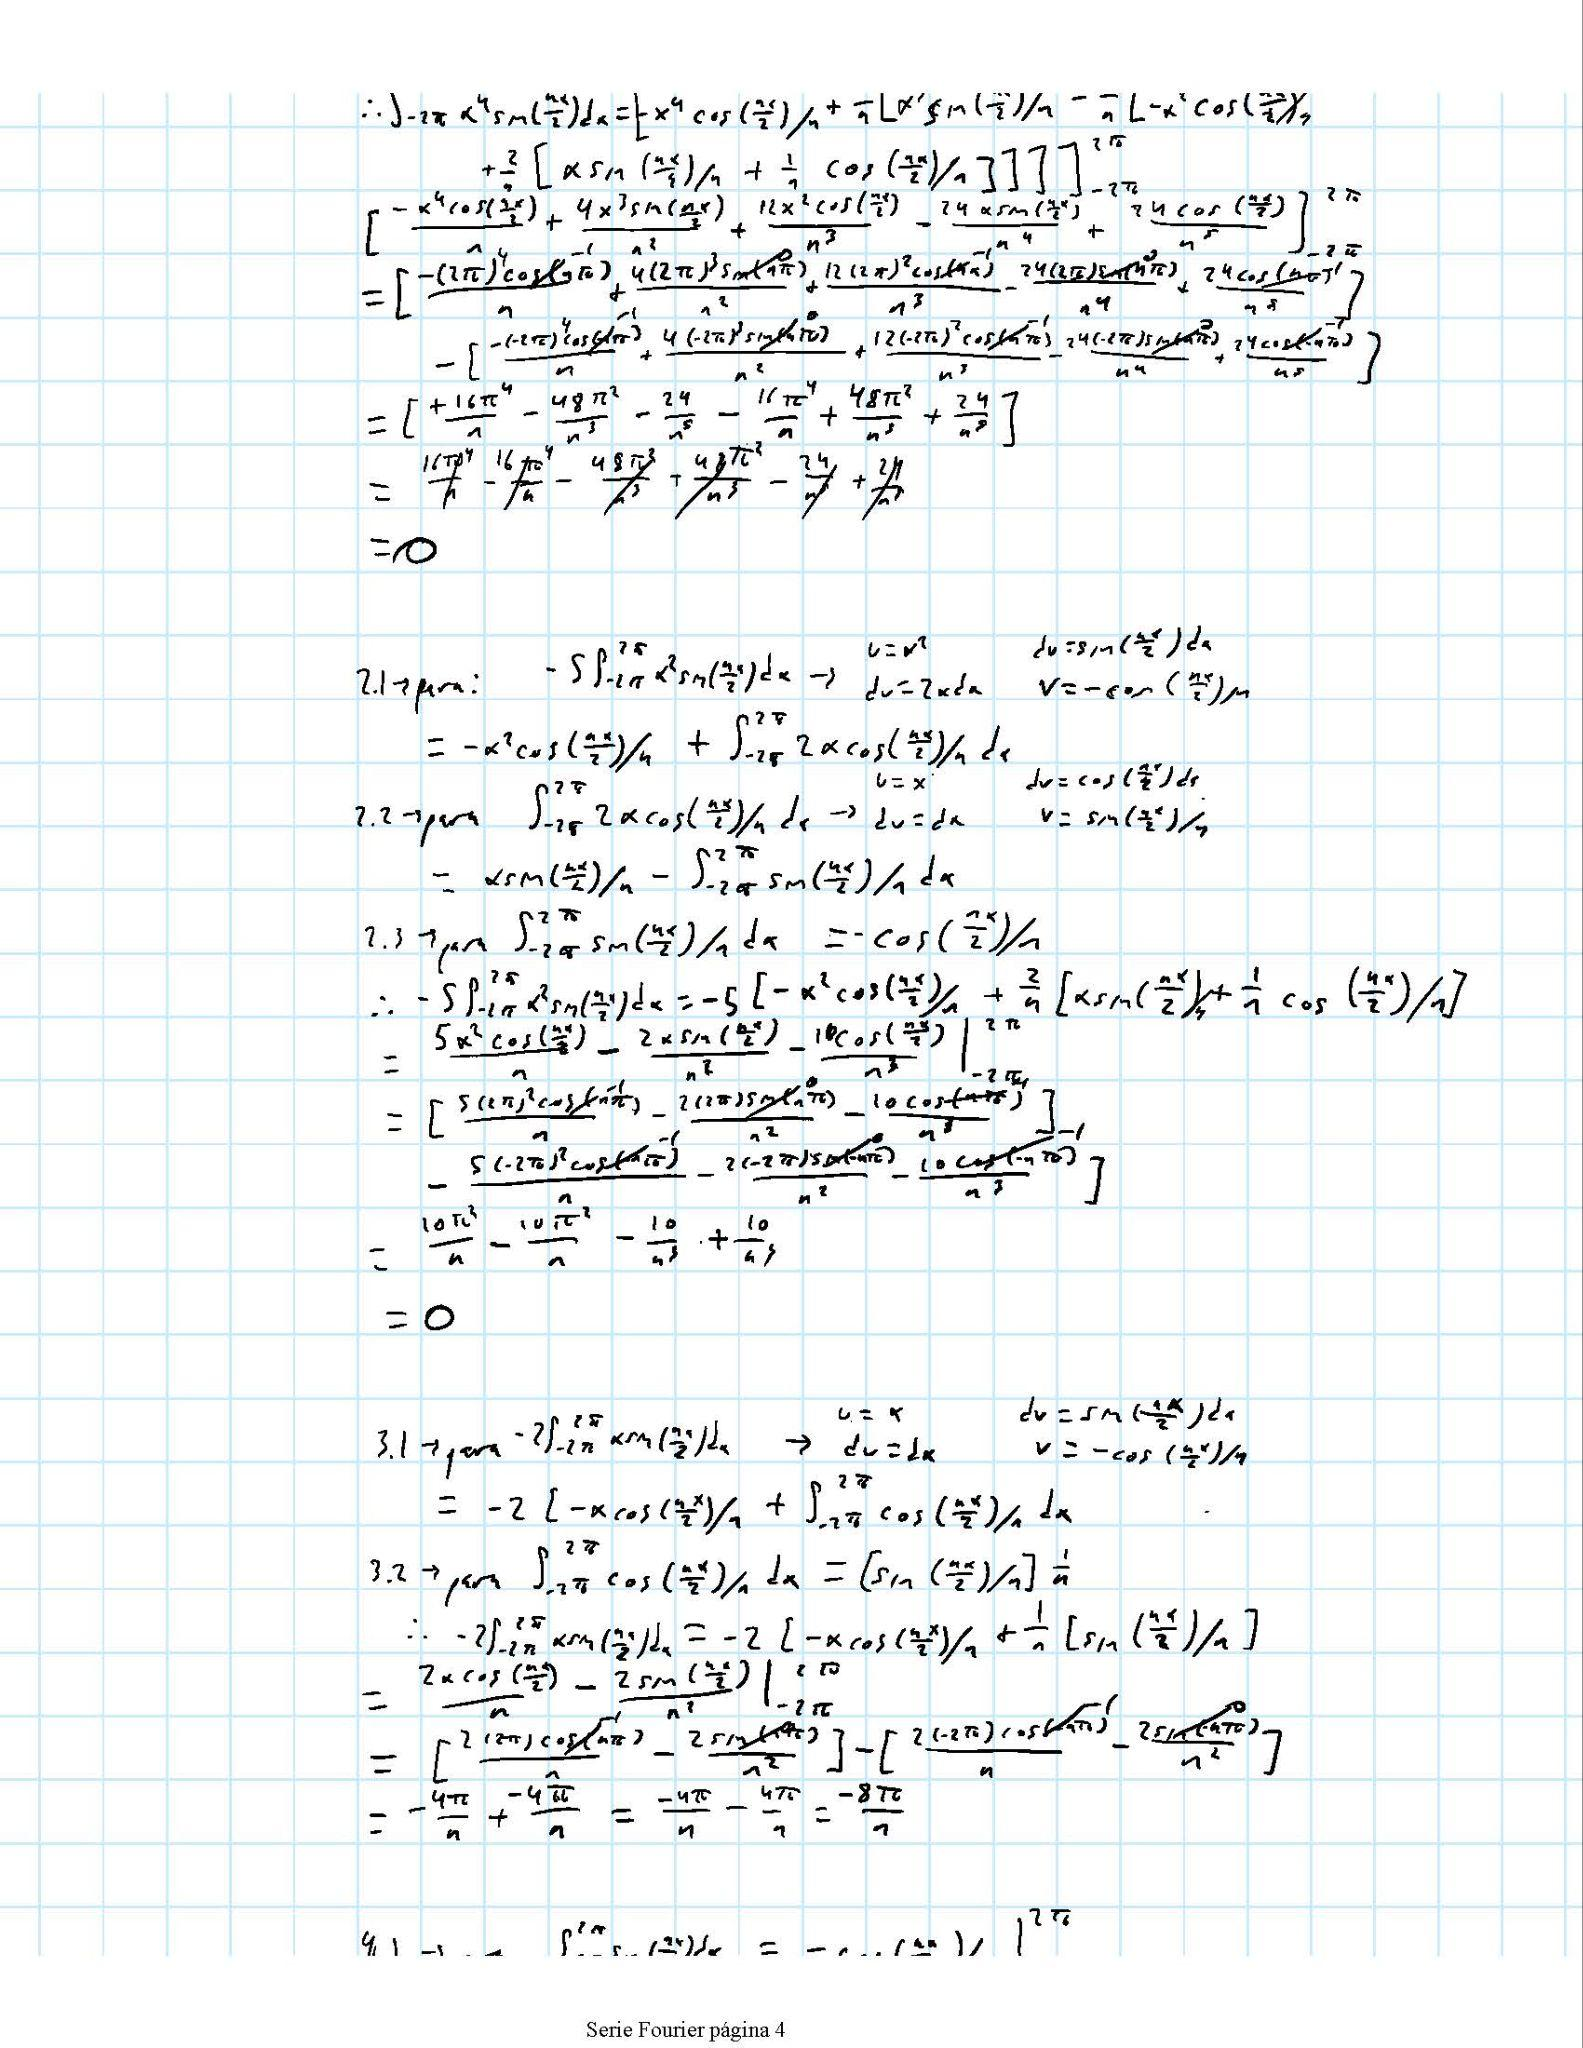
\includegraphics[width=6.26772in,height=8.11111in]{media/image57.jpg}

Imagen 4D. Procedimiento de Fourier

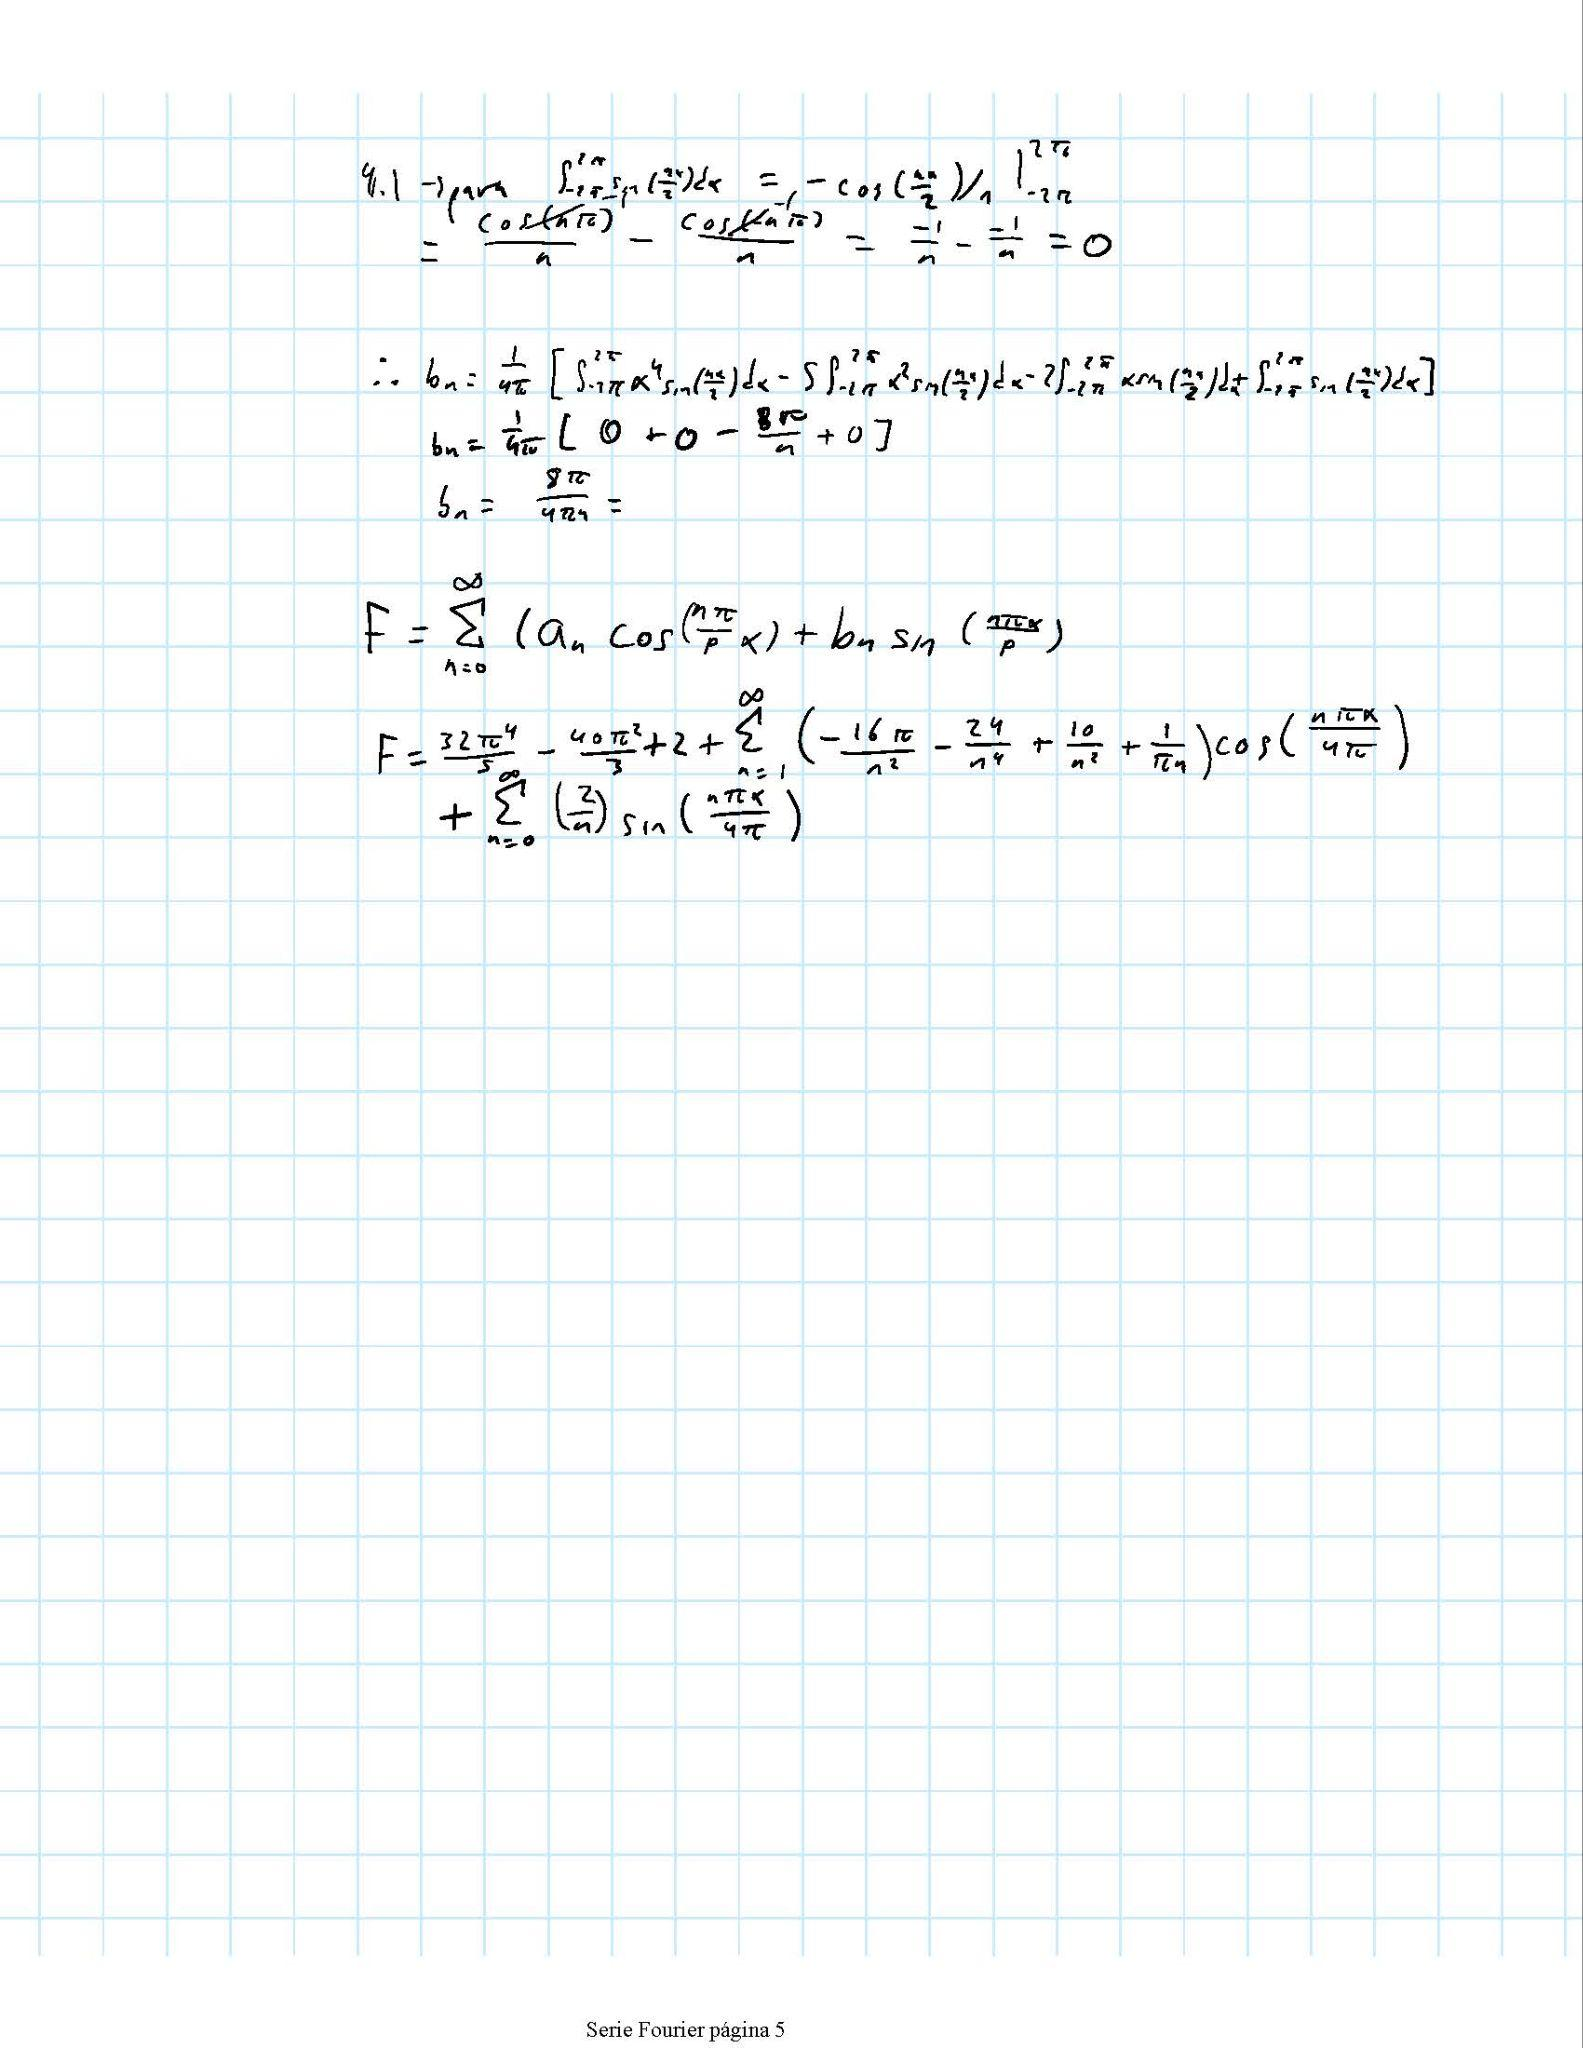
\includegraphics[width=6.26772in,height=8.11111in]{media/image58.jpg}

Imagen 5D. Procedimiento de Fourier
